%This file is just a wrapper. Please, edit the files for your chapter in chapters/chapter1/.
%Don't worry, we will put your chapter in the correct place when assemble the book.

\documentclass[krantz1,ChapterTOCs]{krantz}
\usepackage{fixltx2e,fix-cm}
\usepackage{amssymb}
\usepackage{amsmath}
\usepackage{graphicx}
\usepackage{subfigure}
\usepackage{makeidx}
\usepackage{multicol}

%\usepackage[dvips]{hyperref}

\frenchspacing
\tolerance=5000

\makeindex

\include{frontmatter/preamble} %place custom commands and macros here

\begin{document}

\frontmatter

\title{The Black Book of Quantum Physics\\
%in Socio-Environmental Systems, Public Health, and Insurance\\
{\large(or Bad Maths that Gets the Right Answer)}
}
\author{Cooper Doyle}

\maketitle

%\include{frontmatter/dedication}
%\cleardoublepage
\setcounter{page}{2} %previous pages will be reserved for frontmatter to be added in later.
\tableofcontents
%\include{frontmatter/foreword}
%\include{frontmatter/preface}
%\listoffigures
%\listoftables
%\include{frontmatter/contributor}
%\include{frontmatter/symbollist}

\mainmatter

\part{Introduction}

In the beginning there was nothing. No-one really knows what happened after that, and many people find this deeply unsatisfying. I suppose the meaning of their lives must somehow be tied to something that happened sixteen billion years ago. But we are not going to talk about how we got here. We are going to talk about what is.
As a physicist who has spent many years trying to figure that out, the most satisfying answer I have found is this: reality is an endless fabric of interacting fields, infinite arrays of infinitesimal coupled oscillators, little tiny masses on springs. What follows is an explanation of what that means, and why physicists think it's true.
We will need two experimental results, to be precise — Planck's quantisation, and Born's rule — and to following the logic wherever it goes. A spring, some symmetry arguments, and a deep discomfort with ugly equations. That's the whole of modern physics.
Most courses bury you in experimental evidence before you're allowed to see the theory. This is historically honest but pedagogically backwards — it makes quantum mechanics look like a collection of weird facts rather than an inevitable logical structure. If you take classical mechanics seriously enough, quantum mechanics isn't a shocking departure. It's the destination.
This book is based on my notes as a grad student, and by the end you will not be an expert. But you will be qualified — genuinely qualified — to appreciate just how strange the universe is. Not because Bill Nye told you it is strange, but because you followed the logic yourself, all the way to the edge, and watched it dissolve into something irreducible.
This is not what a mathematician would consider rigorous. But we don't need to worry ourselves with the opinions of mathematicians. We are physicists, after all, and infinity, to us, is just a large number.

%\include{chapters/chapter1/ch1}
%\include{chapters/chapter2/ch2}

\part{The Mechanics of Heaven and Earth}

Mechanics is concerned with two things: matter and energy. Matter is the stuff the universe is shaped out of, while energy is the essence that makes it move. Energy, like matter, comes in many forms: anything that changes, stirs or stops in the world is the result of energy in metamorphosis. Concentrations of energy generate forces that counteract the concentration, leading to the creation of energy of a different type. This interplay continues until equilibrium is achieved. Simple really.\\

We've all heard of Isaac Newton, and we've all heard the story of the Apple. The mass of the Earth creates a concentration of potential energy in the Apple, which generates a gravitational force pulling it to the ground - acting to reduce that potential - which in turn creates kinetic energy by setting the apple in motion.\\

What Isaac Newton actually discovered was that the gravity on earth was the same gravity that governs stars - that pulls planets into orbits around them and pulls them around the milky way. Newton discovered that the mechanics of heaven and earth are the same.\\

This was not obvious. To prove it, Newton had to invent calculus.\\

If we want to understand how all this comes together, how physicists describe the mechanics of heaven and earth, it's good to start with one of the few systems that we can actually solve exactly. It's something known as the simple harmonic oscillator, or the SHO amongst friends, but as all good students of physics know, all that means is a mass on a spring.\\

\section*{A Mass on a Spring}

\begin{figure}[h]
\centering
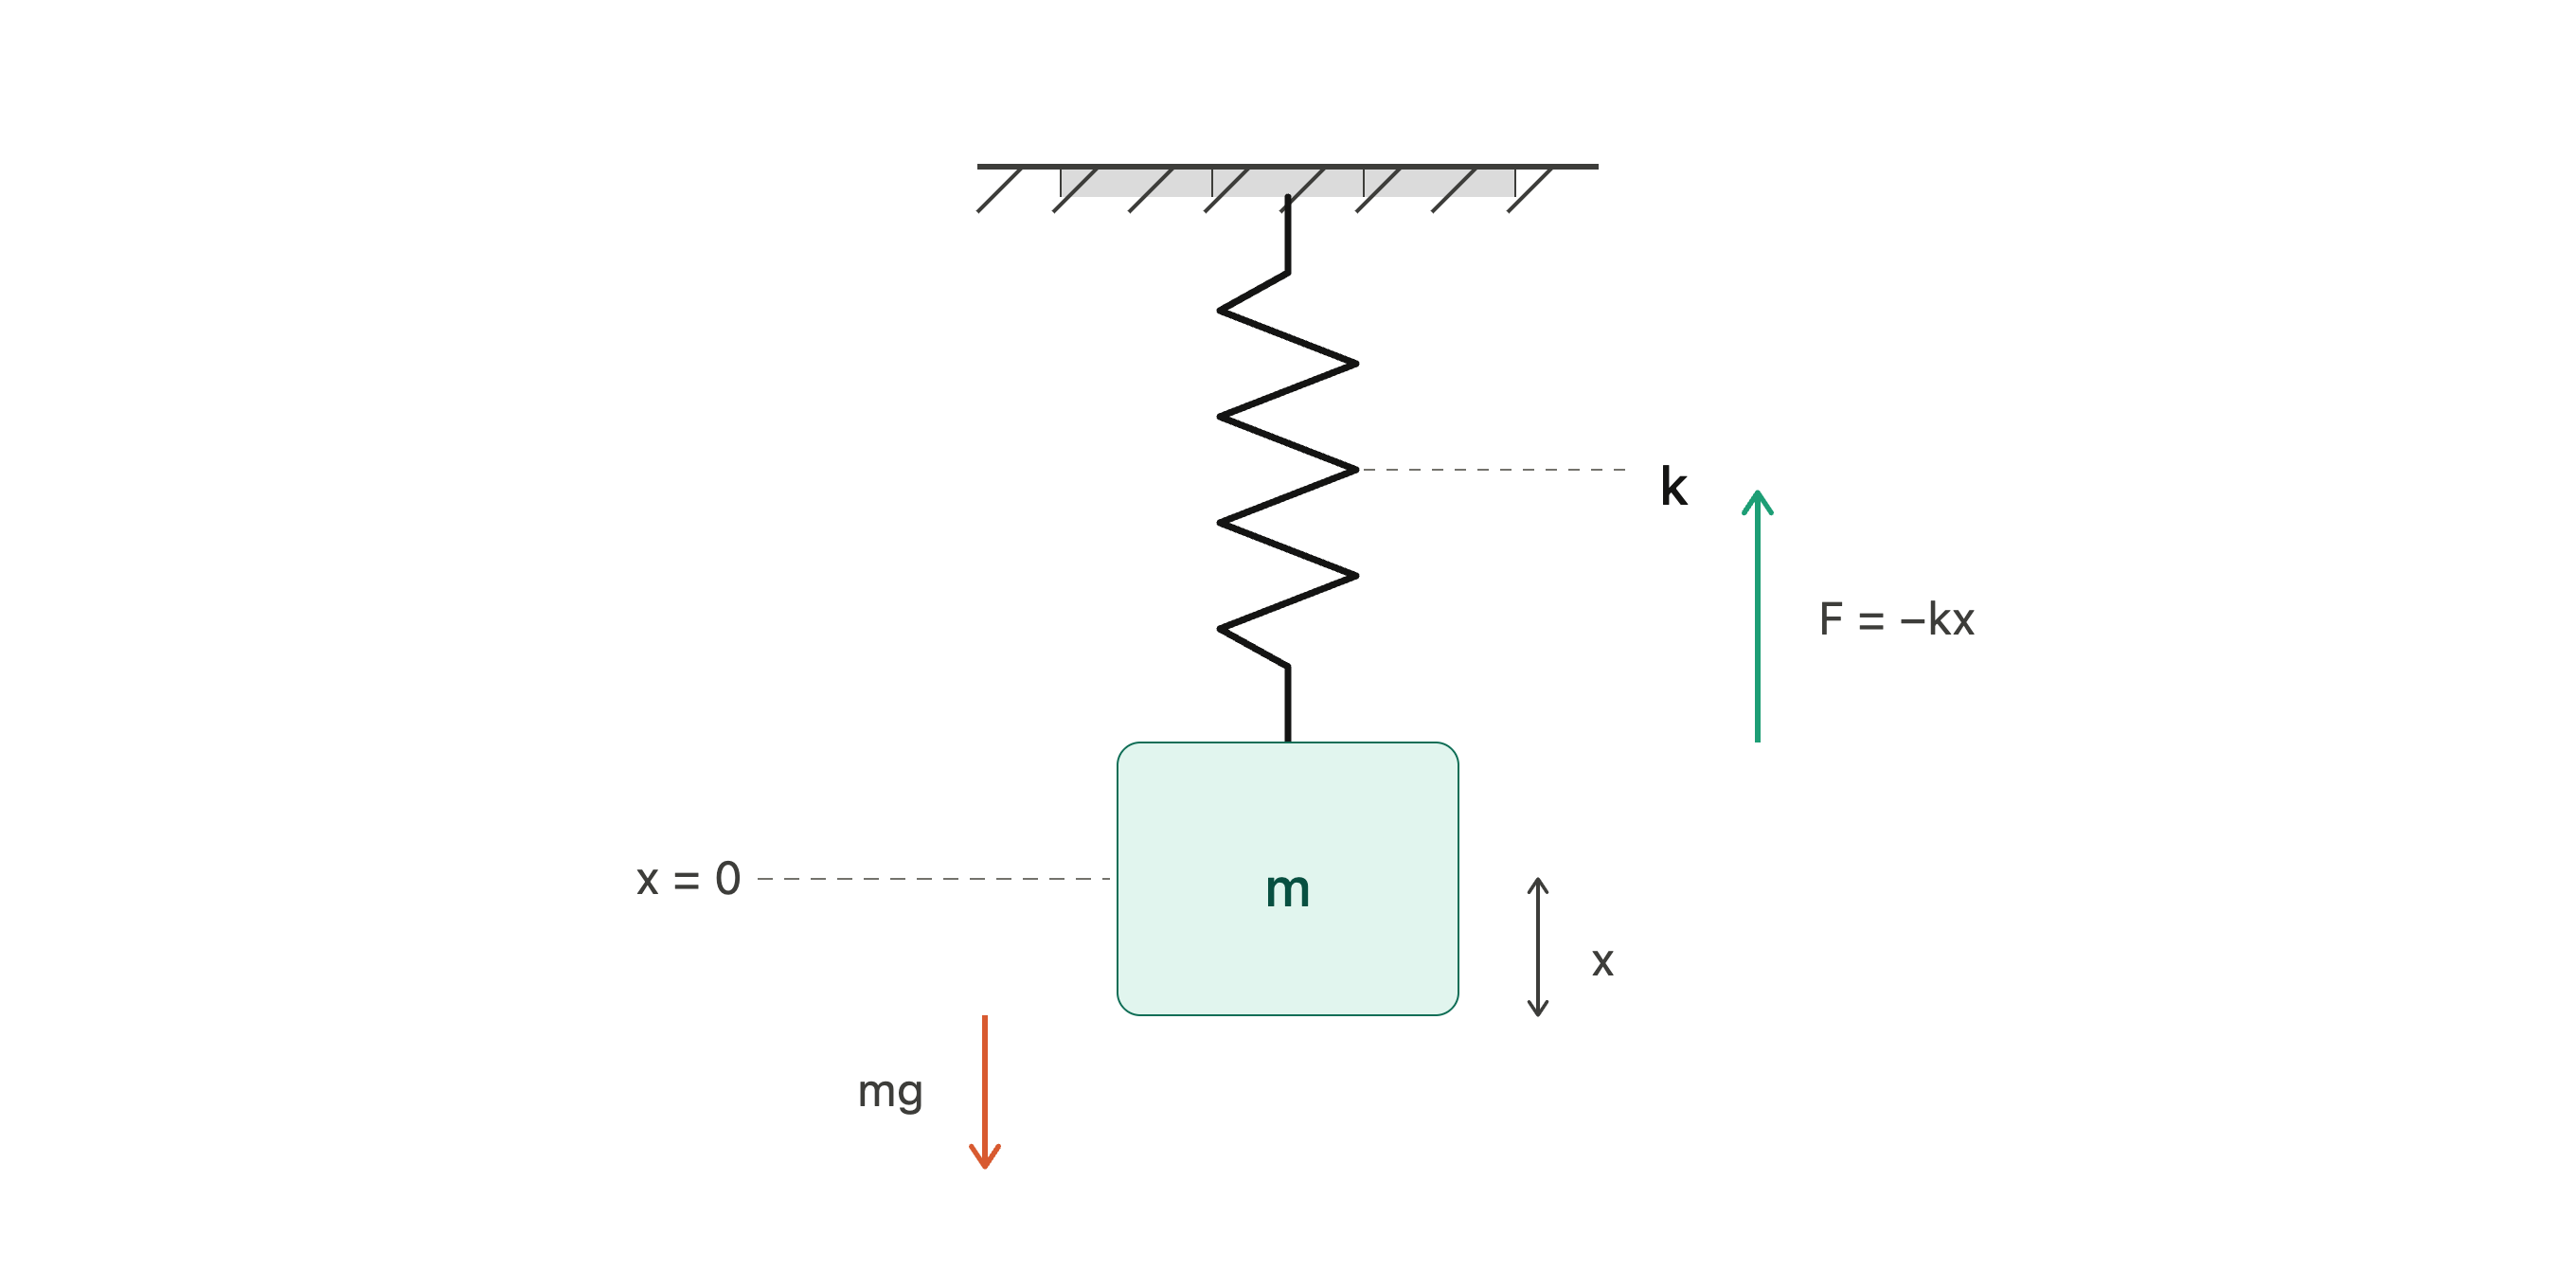
\includegraphics[width=1\textwidth]{img/mass_on_spring_static.png}
\caption{A mass $m$ suspended from a spring of stiffness $k$. The restoring force $F = -kx$ opposes displacement from equilibrium.}
\label{fig:sho}
\end{figure}

Now, the spring doesn't have to be a spring, of course: it could be the gravitational curvature of spacetime caused by a supermassive black star, for example, but we can keep it simple. For physicists the question is this: how do we describe the motion of the mass as a function of time $x(t)$?\\

The standard procedure, according to Newton, would be to first require that the displacement $x$ be zero while the spring is at rest. This will allow us to avoid having to add "$+x_0$ at the end of everything. We can then write down Hooke's law $F=-kx$, which relates the force to the displacement via the stiffness of the spring $k$.\\

The coup de grace is Newton's second and most famous law, $F=ma$, which relates the force of the spring to the acceleration of the mass. We can combine these two laws to get:

$$\ddot{x} = -\frac{k}{m}x$$

where $\ddot{x}$ is shorthand for the acceleration $a=\frac{\delta^2x}{\delta t^2}$. Since the acceleration is the rate of change of the velocity, and the velocity is the rate of change of the position, the acceleration is the rate of change of the rate of change of the position $x$.\\

This is the dynamics equation for the harmonic oscillator. All it says is that at all times $t$ the acceleration $\ddot{x}(t)$ is proportional yet opposite to the displacement $x$ by a constant fraction $\frac{k}{m}$. The further the displacement, the greater the acceleration back to the centre.\\

This tells us everything we need to know about the flow of the system with time, given any initial conditions. While this is good, what we really want isn't the flow: we want to know the trajectory - some function of the position $x(t)$ over time that solves this second order partial differential equation.\\

If you remember your calculus you remember that can get pretty complicated pretty quick. If we're clever we can solve it by simple inspection.\\

After a long stare, we might remember that this is physics and the numbers mean something: they represent a ball on a spring. If we've ever observed a mass on a spring, we might notice that neither the acceleration $\ddot{x}$ nor the position $x$ can run away to infinity: the spring will always pull it back to the centre. So we need our function $x(t)$ to be bounded and periodic, limited in its range and recurring in nature.\\

So we posit some function of the form $x(t)\sim\cos{\omega t+ \phi}$. This is the general function for a wave with $\omega$ as the frequency, and we've added $\phi$ to account for the phase of the wave. If we put this into the above equation we can fill in the gaps to get:

$$x(t)=A\cos{\sqrt{\frac{k}{m}} t + \phi}$$

As we can (and should) check, this solves the original equation. The harmonic oscillator has wave-like solutions with frequency $\omega = \sqrt{\frac{k}{m}}$ driven by the strength of the spring $k$ and dampened by the inertia of the mass $m$. While a spring behaves a bit differently to gravity, this is basically what Newton discovered.\\

This approach is what we call Newtonian physics - a system that worked just fine for many years until some nosy mathematicians from down the hall had to spoil everything.

The fact is, Newtonian physics is extremely un-satisfying as a mathematical system because we have to introduce the intermediary concept of force, which isn't really a fundamental concept. It's an emergent phenomenon, more like a sensation. For example, if we swing a heavy object in circles, we feel a force pulling it away – what's called a centrifugal force. But we know this force isn't actually real; it's a result of the object's tendency to move in a straight line due to its momentum (Newton's first law), combined with the fact that we're forcing it to move in a circle.\\

Not only is force not a fundamental concept, but it also complicates our understanding of interactions, requiring additional assumptions and abstractions that detract from the elegance and simplicity sought in a more foundational theory. Instead, the mathematicians decided that they would describe systems in terms of the {\it action}, which they argued it would seek to stabilise at all costs as it evolved.\\

The first of these mathematicians was Lagrange, and he would express the instantaneous action in terms of something we call the Lagrangian:

$$L = K - U$$

Where K is the kinetic energy of the mass, and U is the potential energy of the spring. Since the mass sits at $x=0$ when the spring is at rest we can write these two explicitly:

$$L = \frac{1}{2}m\dot{x}^2 - \frac{1}{2}kx^2$$

Unsurprisingly, Lagrange would use something called the Euler-Lagrange equations, that assume the system preserves a stationary action as it evolves, to find the path $x(t)$. It turns out this works well.\\

The second of these mathematicians was Hamilton, and he found a somewhat fancier method, using a Legendre transform of the Lagrangian to express the energy in terms of the momentum $p$:

$$H = p\dot{x} - L$$

This was predictably called the Hamiltonian, which represents the total energy of the system. In a way, the Legendre transform translates between action and energy.

$$H = \frac{1}{2m}p^2 + \frac{1}{2}kx^2$$

Or, $H = K + U$. We already know from Newtonian mechanics that the energy, like the action, should also be stationary. Hamilton's coup de grace was Hamilton's equation, which allows us to find $x(t)$.

\begin{equation}
  \left\{\begin{array}{@{}l@{}}
    \dot{x}=\frac{\partial H}{\partial p} = \frac{p}{m} \\
    \dot{p}=\frac{\partial H}{\partial x} = -kx
  \end{array}\right.\,.
\end{equation}

Now we can put all this together and we get:

$$\ddot{x} + \frac{k}{m}x = 0$$

Which is the dynamics equation we solved before. How good! But if the equations are the same, what was the point of all that?\\

In Hamiltonian mechanics we deal directly with energy, which, alongside matter, is one of the most fundamental concepts in physics. The real beauty in these equations is that the flow of the system with time stems directly from an expression of energy.\\

Even more interesting is the Lagrangian mechanics from which the Hamiltonian is derived: we discover a new concept, the action, that turns out to be the invisible hand that guides the mechanics of heaven and earth. We have condensed Newton's principles into one handy statement:\\

``\textit{The path taken by a system between two states is the one for which the action is minimized"}\\

In fact, let's think about our heavy object - why is it that it wants to conserve its momentum? For Newton this reality is simply stated as an empirical law. No explanation needed. For Hamilton, this is a direct consequence of the Hamiltonian itself!\\

Noether's theorem, invented by Emmy Noether, one of the great unsung heroes of physics and mathematics, tells us that the conserved momentum is the result of symmetries in the Hamiltonian. Say, for instance, we remove the spring from our simple harmonic oscillator. The Hamiltonian becomes:

$$H = \frac{1}{2m}p^2$$

Now the energy is independent of $x$ - the Hamiltonian is symmetric with respect to translations in the $x$ direction. Noether's theorem tells us that this symmetry produces a conserved quantity: the momentum in the $x$ direction. This is because a constant momentum translates to a stable action - which, if you remember, was how we got into this mess in the first place.\\

So Newton's first law is a special case where the Hamiltonian is translationally symmetric, and the corresponding conserved quantity is the momentum. Our Simple Harmonic Oscillator is symmetric about $x=0$, and our conserved quantity is the frequency of the periodic path.\\

With the work of Lagrange, Hamilton and Noether, classical physicists had settled back into their confidence. It seemed there was nothing that could shake their theories, and that a comprehensive theory of nature was probably just a few equations away.\\

The universe still had a few tricks up its sleeve.\\

\section*{What is a Field? Begin with a Spring.}

We have spent considerable time with a single mass on a single spring. 
But the universe is not made of single masses on single springs. It is 
made of vast collections of things, all pushing and pulling on each 
other simultaneously. So let us ask: what happens when we take our 
simple harmonic oscillator and replicate it infinitely?\\

Imagine a long chain of identical masses, each one connected to its 
neighbours by springs of stiffness $k$. Each mass wants to sit at its 
equilibrium position, but it is enslaved to its neighbours --- if one 
moves, it drags the others with it. The Hamiltonian for the whole chain 
is just the sum over all the individual oscillators, with extra terms 
for the energy stored in the coupling between neighbours:

\begin{equation}
H = \sum_{n} \left[ \frac{1}{2m} p_n^2 + \frac{k}{2} \left( x_n - 
x_{n-1} \right)^2 + \frac{k}{2} \left( x_{n+1} - x_n \right)^2 \right]
\end{equation}

The first term is the kinetic energy of each mass. The second and third 
are the potential energy stored in each spring, which depends only on 
the relative displacement of neighbouring masses. Hamilton's equations 
give us:

\begin{equation}
\dot{x}_n = \frac{\partial H}{\partial p_n} = \frac{p_n}{m}
\end{equation}

\begin{equation}
\dot{p}_n = -\frac{\partial H}{\partial x_n} = 2k \left( x_{n-1} - 
x_n \right) + 2k \left( x_{n+1} - x_n \right)
\end{equation}

\begin{equation}
\therefore \ddot{x}_n = \frac{2k}{m} \left( x_{n-1} + x_{n+1} - 
2x_n \right)
\end{equation}

This says something physically transparent: the acceleration of each 
mass depends on how far it sits above or below its two neighbours. If 
it is higher than both, they pull it down. If it is lower, they push 
it up. The motion of each mass is completely determined by the 
configuration of the whole chain.\\

We know from the single oscillator that solutions must be periodic in 
time. But now we have a spatial degree of freedom too --- the index $n$ 
--- and the solutions must organise themselves across the whole chain. 
We write:

\begin{equation}
x_j(t) = A_j\, e^{i(\omega t + \phi)}
\end{equation}

But unlike before, we cannot simply read off the amplitude. The spatial 
component $A_j$ has to be deduced from the structure of the chain 
itself. This is where things get interesting.\\

\section*{Continuum Limit --- The Wave Equation}

Rather than solving the discrete problem, we do something physicists 
love and mathematicians tolerate: we take the limit as the spacing 
between masses $\delta x$ goes to zero, and the discrete chain becomes 
a continuous medium. We label each mass by its equilibrium position 
$n\delta x$ and replace the discrete displacements $x_n(t)$ with a 
smooth function $\psi(x, t)$.\\

The equation of motion becomes:

\begin{equation}
\frac{\partial^2 \psi(x,t)}{\partial t^2} = \frac{k}{m} \left[ 
\psi(x+\delta x,t) - 2\psi(x,t) + \psi(x - \delta x, t) \right] 
\frac{1}{\delta x}
\end{equation}

The bracketed expression is just the finite difference approximation 
to the second spatial derivative. As $\delta x \to 0$ it becomes exact, 
and substituting the mass density $\mu = \frac{m}{\delta x}$ and 
elastic modulus $E = k\delta x$:

\begin{equation}
\frac{\partial^2 \psi(x,t)}{\partial t^2} = \frac{E}{\mu} 
\frac{\partial^2 \psi(x,t)}{\partial x^2}
\end{equation}

This is the wave equation. It emerged from nothing more exotic than a 
chain of springs and a willingness to take a limit. The solutions are 
waves propagating through the medium:

\begin{equation}
\psi(x,t) = e^{ikx}\, e^{i\omega t}
\end{equation}

with phase velocity:

\begin{equation}
v = \frac{\omega}{k} = \sqrt{\frac{E}{\mu}}
\end{equation}

We started with a mass on a spring and ended up with a propagating 
wave. The spring is still there --- it is just that when you have 
infinitely many of them, the collective behaviour is no longer 
oscillation. It is propagation. This is what a field is: an infinite 
array of coupled oscillators, and its natural language is waves.\\

And this, it turns out, is not merely a mechanical curiosity.\\

\part{Light}

Harmonic Oscillator

In Newton's classical mechanics we described the motion of a simple harmonic oscillator using the force exerted on it from spring. What you might notice is that in Hamiltonian mechanics, we don't need the spring. Instead we think of a potential that exists everywhere along a line (parametrised by $x$), which is quadratic in $x$. The force exerted on the object is the slope of the potential, pulling the mass towards a minimum at the origin.\\

This trick is particularly useful when we look beyond springs. The potential could be caused by a mass, a magnet or an electric charge - it's what we would call a field. It's a way to describe the influence of forces at every point in space, not just at the position of the mass. Or, more precisely, it's a way to describe the energy of a system's configuration at any point in time.\\

James Clerk Maxwell was a pioneer in studying fields in the context of electromagnetism. He developed equations that describe how electric and magnetic fields interact and propagate, and he narrowed them down to just 4.\\

The first equation is Gauss's law for electricity:

\[
\nabla \cdot \mathbf{E} = \frac{\rho}{\epsilon_0}
\]

The electric field \(\mathbf{E}\) is the negative gradient of the electric potential \(V\):

\[
\mathbf{E} = -\nabla V
\]

It's a field that relates a force vector to every point in three dimensional space. The divergence $\nabla \cdot \mathbf{E}$ is a way to measure the "spread" or "flow" of the field. It tells us how the electric field originates from charges and radiates uniformly outward, in proportion to the charge density \(\rho\) and divided by the permittivity of free space \(\epsilon_0\).\\

It's a nice rule of thumb that fields like this, in three dimensional space, the strength of the field decreases as the squared distance from the charge or mass, since the field density spreads out like the surface of a sphere that expands outwards with the radius.\\

\[
E = \frac{Q}{4\pi \epsilon_0 r^2}
\]

The second equation is Gauss's law for magnetism:

\[
\nabla \cdot \mathbf{B} = 0
\]

This says there are no magnetic monopoles; magnetic fields don't start or end at any point. Imagine a river with magnetic field lines as water currents. The currents never start or stop abruptly; they flow continuously in loops.\\

The third equation is Faraday's law of induction:

\begin{equation}
\nabla \times \mathbf{E} = -\frac{\partial \mathbf{B}}{\partial t}
\end{equation}

Which explains how a changing magnetic field creates an electric field. $\nabla \times \mathbf{E}$ is the curl, which measures the \textit{rotation} of the field. So moving a magnet creates a rotating electric field.\\

The fourth equation is Ampère's law (with Maxwell's addition):

\[
\nabla \times \mathbf{B} = \mu_0 \mathbf{J} + \mu_0 \epsilon_0 \frac{\partial \mathbf{E}}{\partial t}
\]

Which says electric currents and changing electric fields will also create magnetic fields.\\

To understand the profound implications of Maxwell's equations, let’s derive the wave equation for electromagnetic waves, showing how they predict the propagation of light. By taking the curl of Faraday's law (\(\nabla \times \mathbf{E} = -\frac{\partial \mathbf{B}}{\partial t}\)) and using the vector identity \(\nabla \times (\nabla \times \mathbf{E}) = \nabla (\nabla \cdot \mathbf{E}) - \nabla^2 \mathbf{E}\), we get:

\[
\nabla \times (\nabla \times \mathbf{E}) = \nabla (\nabla \cdot \mathbf{E}) - \nabla^2 \mathbf{E} = -\frac{\partial}{\partial t} (\nabla \times \mathbf{B})
\]

Using Gauss's law (\(\nabla \cdot \mathbf{E} = \frac{\rho}{\epsilon_0}\)), for free space where \(\rho = 0\), we have \(\nabla \cdot \mathbf{E} = 0\). Thus, \(\nabla \times (\nabla \times \mathbf{E}) = -\nabla^2 \mathbf{E}\).\\

Substituting Ampère's law (\(\nabla \times \mathbf{B} = \mu_0 \epsilon_0 \frac{\partial \mathbf{E}}{\partial t}\)) into the above equation, we get:

\[
-\nabla^2 \mathbf{E} = -\mu_0 \epsilon_0 \frac{\partial^2 \mathbf{E}}{\partial t^2}
\]

This simplifies to the wave equation for the electric field:

\[
\nabla^2 \mathbf{E} = \mu_0 \epsilon_0 \frac{\partial^2 \mathbf{E}}{\partial t^2}
\]

A similar derivation can be done for the magnetic field, yielding:

\[
\nabla^2 \mathbf{B} = \mu_0 \epsilon_0 \frac{\partial^2 \mathbf{B}}{\partial t^2}
\]

These are the wave equations for electromagnetic waves, predicting that changes in the electric and magnetic fields propagate through space as waves at the speed of light \( c = \frac{1}{\sqrt{\mu_0 \epsilon_0}} \).\\

One of the most profound insights from Maxwell's equations came when Einstein considered their implications. He realized that the speed of light must be constant, independent of the motion of the observer. This realization was a cornerstone of his theory of special relativity, which revolutionized our understanding of space and time.\\

The interplay between fields, particles, and the speed of light set the stage for the next great leap in physics, bridging classical mechanics and modern physics.


\part{The Jacobi Conspiracy}

There is a thread running through classical mechanics that nobody told you about in school. It connects a mass on a spring to the propagation of light, and from there to the structure of quantum mechanics itself. Jacobi found it, sat on it for half a century, and the rest of physics took that long to catch up.\\

The conspiracy begins, as all good conspiracies do, with something completely innocent.\\

We already know that an infinite chain of coupled springs, in the continuum limit, produces the wave equation. We did that at the end of the last chapter and it felt like a nice result --- mechanics gives rise to waves. Good. But now ask a different question. What else has this shape?\\

\section*{Optical Fields --- The LC Circuit}

Consider the humble LC circuit: a series inductor and capacitor.

\begin{figure}[h]
\centering
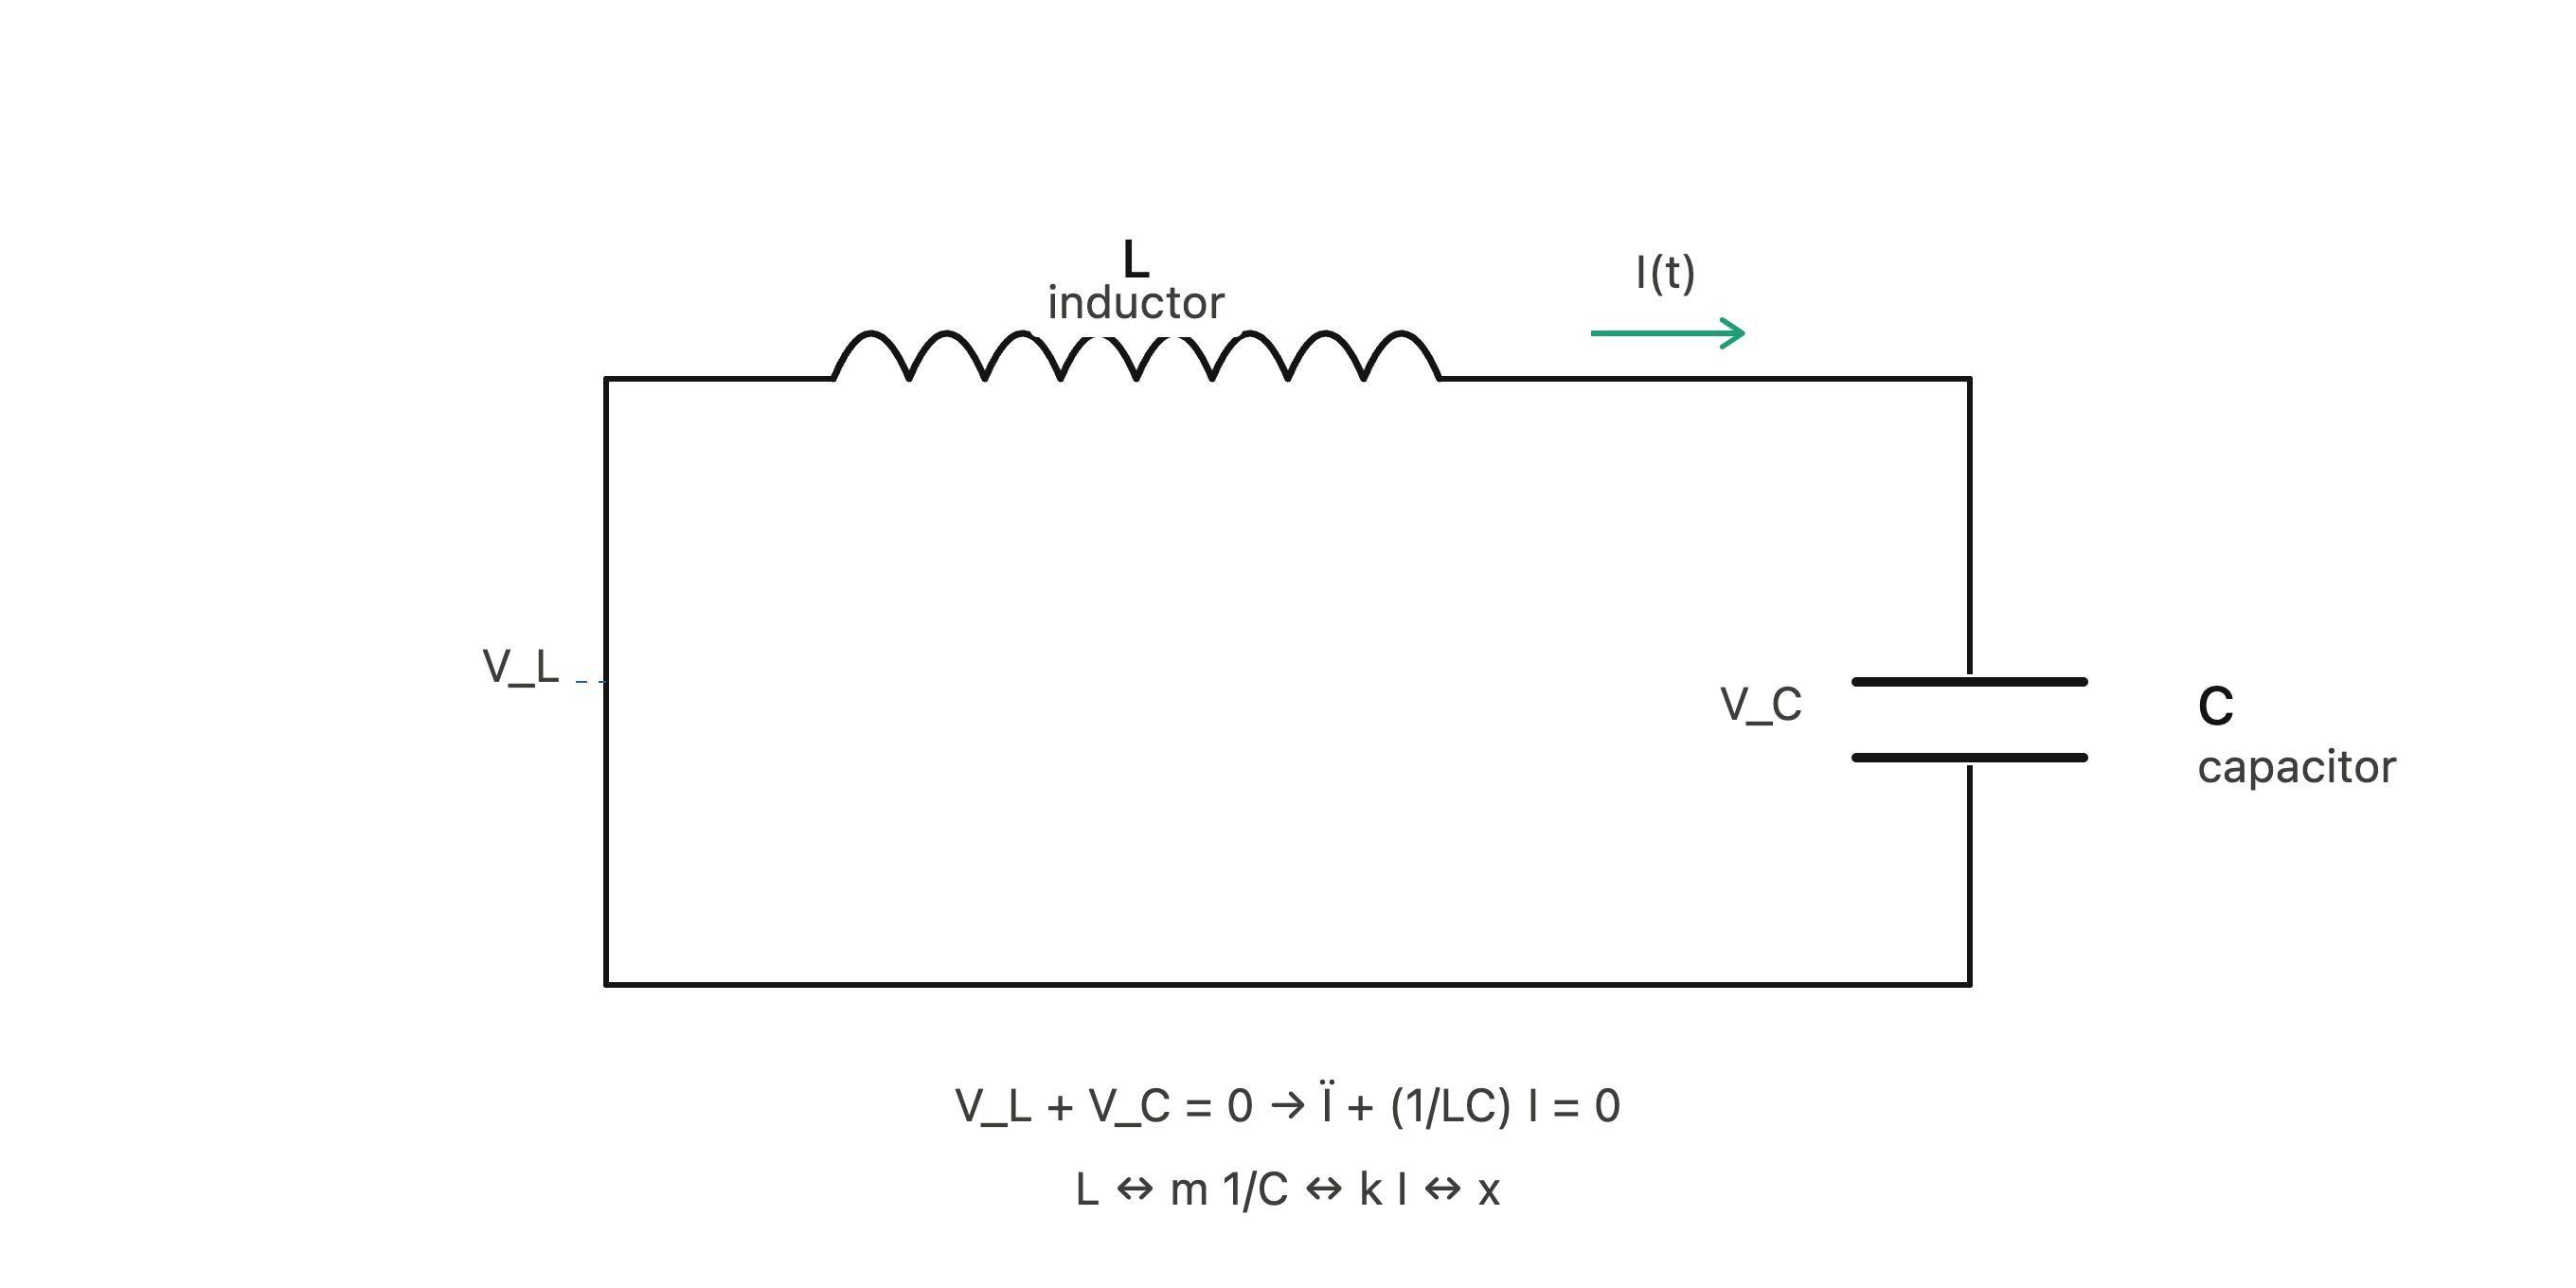
\includegraphics[width=1\textwidth]{img/LC_circuit_static.png}
\caption{A series LC circuit. The inductor $L$ plays the role of the mass and the capacitor $C$ plays the role of the spring, with the exact correspondence $L \leftrightarrow m$ and $1/C \leftrightarrow k$.}
\label{fig:lc}
\end{figure}

Nothing exotic. Kirchhoff's laws give us:

$$V_C + V_L = 0 \qquad I_C = I_L$$

With the constitutive relations for each component:

$$V_L(t) = L\frac{dI_L}{dt} \qquad I_C(t) = C\frac{dV_C}{dt}$$

Combining these, the current satisfies:

$$\frac{d^2}{dt^2}I(t) + \frac{1}{LC}I(t) = 0$$

This is identical to the equation of motion for a mass on a spring, with the substitution $\frac{k}{m} \to \frac{1}{LC}$. The capacitor plays the role of the spring --- storing energy in an electric field --- and the inductor plays the role of the mass, resisting changes in current through its inertia. The complementarity is exact:

$$k \leftrightarrow \frac{1}{C} \qquad m \leftrightarrow L$$

The solutions are identical too:

$$I(t) = C_1\cos\omega t + C_2\sin\omega t, \qquad \omega = \frac{1}{\sqrt{LC}}$$

An LC circuit is just a mass on a spring. It oscillates for exactly the same reason, described by exactly the same equation. This is either a remarkable coincidence or a hint that something deeper is going on.\\

It is not a coincidence.\\

\section*{Collective Excitations of an Infinite LC Array}

Just as we strung together an infinite chain of mechanical oscillators to get the wave equation, we can do the same with LC circuits. Consider an infinite transmission line --- inductors in series, capacitors to ground, repeating forever. The voltage and current satisfy:

$$V(x) - V(x+\delta x) = L\,\delta x\,\frac{\partial I}{\partial t}$$

$$I(x) - I(x+\delta x) = C\,\delta x\,\frac{\partial V}{\partial t}$$

Taking the continuum limit $\delta x \to 0$ and combining:

$$\frac{\partial^2 V}{\partial x^2} = LC\frac{\partial^2 V}{\partial t^2}$$

Now substitute the electric permittivity $\varepsilon = C\,\delta x$ and magnetic permeability $\mu = L\,\delta x$:

$$\frac{\partial^2 V}{\partial x^2} = \mu\varepsilon\frac{\partial^2 V}{\partial t^2}$$

The wave equation again. Solutions are propagating exponentials:

$$V(x,t) = e^{ikx}e^{i\omega t}, \qquad v = \frac{d\omega}{dk} = \frac{1}{\sqrt{\mu\varepsilon}}$$

\section*{Classical Field Theory}

Now for the punchline. Take $\mu = \mu_0$ and $\varepsilon = \varepsilon_0$ --- the permeability and permittivity of free space. The phase velocity becomes:

$$v = \frac{1}{\sqrt{\mu_0\varepsilon_0}} = c$$

The speed of light. Out of a transmission line.\\

This is not a trick. The electromagnetic field in free space is, mathematically and physically, an infinite array of coupled LC oscillators --- with the elasticity of the vacuum playing the role of the capacitance and the inertia of the vacuum playing the role of the inductance. We can verify this by going back to Maxwell's equations directly.\\

In free space, with a plane wave propagating in the $z$ direction, Maxwell's four equations collapse to just two:

$$\frac{\partial E_x}{\partial z} = -\frac{\partial B_y}{\partial t} \qquad \frac{\partial B_y}{\partial z} = -\frac{1}{c^2}\frac{\partial E_x}{\partial t}$$

Combining them:

$$\frac{\partial^2 E_x}{\partial z^2} = \frac{1}{c^2}\frac{\partial^2 E_x}{\partial t^2}$$

The same wave equation, with the same solutions, and the same speed. Maxwell derived this from the laws of electromagnetism. We derived it from a chain of springs. They are the same equation because they are describing the same thing --- a field, an infinite array of coupled oscillators, rippling through space.\\

This wave propagates at speed $c$ independently of the motion of the source. Not relative to anything --- just $c$, always, everywhere. This is not what Galilean relativity would predict, and it is the first whisper of something that would eventually become Einstein's special relativity. We will return to this in due course.\\

For now, there is a more pressing conspiracy to unravel.\\

\section*{The Conspiracy}

So here is where we stand. We have mechanics --- particles, masses, springs, Hamiltonians. We have fields --- electromagnetic waves, Maxwell's equations, light. And we have just shown that these two things are secretly the same mathematical structure, wearing different clothes.\\

Jacobi had been sitting on an even more unsettling version of this idea. He had noticed that Hamilton's formalism --- the action, the generating functions, the surfaces of constant $S$ --- had a precise optical analogue. That particle trajectories are to mechanics what light rays are to optics. That the principle of least action and Fermat's principle of least time are not just similar in spirit but identical in structure.\\

If fields are waves, and particles live in fields, what are particles?\\

Jacobi's answer, buried in his lectures and largely ignored, was essentially this: particles are waves too. They just don't know it yet.\\

To see why, we need to look more carefully at what Hamilton's equations are actually telling us.\\

\section*{Hamilton--Jacobi Theory}

So by this stage we are pretty sure everything is waves. The 
mechanical field is a wave. The electromagnetic field is a wave. 
Maxwell's equations predicted light as a wave before anyone had 
thought to check. The universe seems to be trying to tell us 
something.\\

Jacobi had been trying to tell us the same thing for half a century, 
and nobody was listening. His insight was this: Hamilton's formalism, 
taken seriously enough, already contains the wave theory of mechanics. 
It has been there all along, hiding in plain sight.\\

To see it, we need to think carefully about what it means to change 
coordinates.\\

\subsection*{Canonical Transformations}

Hamilton's equations have a beautiful structure. The question Jacobi 
asked was: which coordinate transformations preserve that structure? 
If we relabel our positions and momenta --- going from $(q, p)$ to 
some new coordinates $(Q, P)$ --- when do Hamilton's equations still 
hold in the new coordinates?\\

The answer is: when the transformation is \textit{canonical}. These 
are generated by a generating function $F(q, p, Q, P, t)$, which 
relates the old and new coordinates via:

\[
\begin{cases}
p_i = \dfrac{\partial F}{\partial q_i} \quad\text{or}\quad 
q_i = -\dfrac{\partial F}{\partial p_i} \\[8pt]
Q_i = \dfrac{\partial F}{\partial p_i} \quad\text{or}\quad 
P_i = -\dfrac{\partial F}{\partial Q_i}
\end{cases}
\qquad \tilde{H} = H + \frac{\partial F}{\partial t}
\]

The new Hamiltonian $\tilde{H}$ picks up a correction from the 
time-dependence of $F$. A transformation is canonical if:

\[
\frac{\partial p_i}{\partial P_i}\frac{\partial Q_i}{\partial q_i} 
= \frac{\partial^2 F}{\partial P_i\,\partial q_i}
\]

This is a constraint on $F$ that ensures the symplectic structure of 
Hamilton's equations is preserved. The reason to care about this is 
that a clever choice of generating function can make an otherwise 
intractable problem trivial. Jacobi found the cleverest choice of all.\\

\subsection*{Jacobi's Trick}

What if we chose $F$ such that the transformed Hamiltonian vanished 
entirely? If $\tilde{H} = 0$, then Hamilton's equations in the new 
coordinates give $\dot{Q}_i = 0$ and $\dot{P}_i = 0$ --- the new 
coordinates are all constants of motion. The dynamics has been 
completely absorbed into the generating function.\\

Call this generating function $S$. The condition $\tilde{H} = 0$ 
becomes:

\[
\boxed{H\!\left(t,\, q_i,\, \frac{\partial S}{\partial q_i}\right) 
+ \frac{\partial S}{\partial t} = 0}
\]

This is the Hamilton--Jacobi equation. It is a single partial 
differential equation for $S$, and solving it is equivalent to solving 
the full dynamics of the system. All the complexity of the trajectory 
is encoded in one function.\\

For time-independent Hamiltonians, we can separate variables and look 
for a solution of the form:

\[
S = -Et + \sum_i W_i(q_i)
\]

Since $\frac{\partial H}{\partial t} = 0$, the time derivative 
$\frac{\partial S}{\partial t} = -E$ must be constant, which fixes 
the time-dependent part immediately. The momenta are then:

\[
p_i = \frac{\partial S}{\partial q_i} = W_i'(q_i)
\]

\subsection*{A Single Particle in a Potential}

For a single particle of mass $m$ in a potential $V(q)$, the 
Hamiltonian is $H = \frac{1}{2m}p^2 + V(q)$, and the 
Hamilton--Jacobi equation becomes simply:

\[
\boxed{\frac{1}{2m}p^2 + V(q) = E}
\]

Which we recognise immediately as conservation of energy. $E$ is 
just the total energy $K + U$, and we have recovered something we 
already knew by a very long route. This is reassuring. Jacobi's 
machinery is consistent with everything that came before --- it just 
packages it differently.\\

For the harmonic oscillator with $V(q) = \frac{1}{2}kq^2$:

\[
\boxed{\frac{1}{2m}p^2 + \frac{1}{2}kq^2 = E}
\]

This is the equation of an ellipse in phase space --- exactly the 
closed orbits we found before. The momentum at any position is:

\[
p = \sqrt{2m\left(E - \frac{1}{2}kq^2\right)}
\]

And the full generating function is:

\[
S = -Et + \int\sqrt{2m\left(E - \frac{kq^2}{2}\right)}\;dq
\]

In its most general form, for a particle moving in three dimensions:

\[
\boxed{\frac{1}{2m}(\nabla S)^2 + V + \frac{\partial S}{\partial t} 
= 0}
\]

\subsection*{The HJE as a Wave Equation}

Now here is where Jacobi's conspiracy reveals itself.\\

The Hamilton--Jacobi equation is a partial differential equation, 
and its solutions $S$ define surfaces in configuration space --- 
surfaces of constant action, like contour lines on a map. The normal 
to these surfaces points in the direction $\nabla S$, and since:

\[
p_i = \frac{\partial S}{\partial q_i} \qquad \text{or} \qquad 
\vec{p} = \nabla S
\]

the momentum of the particle always points perpendicular to these 
surfaces. The particle trajectory is orthogonal to the surfaces of 
constant $S$.\\

If this sounds familiar, it should. In optics, light rays are 
perpendicular to wavefronts --- surfaces of constant phase $\phi$. 
Fermat's principle says that light takes the path of least time 
between two wavefronts. Hamilton's principle says that particles take 
the path of least action between two surfaces of constant $S$.\\

The analogy is not merely poetic. It is structural. To see this, take 
the total time derivative of $S$ along a trajectory:

\[
\frac{dS}{dt} = \frac{\partial S}{\partial t} + \sum_i 
\frac{\partial S}{\partial q_i}\dot{q}_i
= -H + \sum_i p_i \dot{q}_i = \mathcal{L}
\]

And integrating along the trajectory between times $t_i$ and $t_f$:

\[
\Delta S = S(t_f) - S(t_i) = \int_{t_i}^{t_f} \mathcal{L}\;dt
\]

The change in $S$ between two surfaces is exactly the action 
accumulated along the trajectory. Just as light rays accumulate 
equal phase between wavefronts, particles accumulate equal action 
between surfaces of constant $S$.\\

Particles, in Jacobi's picture, propagate through configuration 
space exactly as light propagates through physical space. The 
generating function $S$ is the mechanical analogue of the optical 
phase. The trajectory is the mechanical analogue of the ray.\\

This is the conspiracy. Mechanics and optics are the same theory, 
written in different variables. And if light --- which we now know 
is a wave --- has this ray description as a limiting case, then 
perhaps mechanics does too. Perhaps the ray picture of particles 
is also just a limiting case of something deeper.\\

Perhaps particles are waves. Planck is about to give us the scale 
at which we find out.\\

\part{Ultraviolet Catastrophe}

By the end of the nineteenth century, classical physics was feeling 
rather pleased with itself. Maxwell had unified electricity and 
magnetism. Hamilton and Jacobi had revealed the deep structure of 
mechanics. The wave theory of light was unassailable. A comprehensive 
theory of nature seemed not just possible but imminent.\\

Then someone looked carefully at a hot oven, and everything fell apart.\\

\section*{Blackbody Radiation}

A blackbody is an idealised object that absorbs all radiation incident 
upon it and emits radiation purely as a function of its temperature. 
A cavity with a small hole is a good approximation --- radiation 
entering the hole bounces around inside until it is absorbed, and the 
light leaking back out carries information only about the temperature 
of the walls.\\

The question classical physics wanted to answer was simple: what is 
the spectral distribution of that radiation? How much energy is emitted 
at each frequency?\\

To answer it, we first need to count the modes. We already know from 
our discussion of fields that a cavity supports standing electromagnetic 
waves --- modes, each with a fixed frequency determined by the 
geometry of the cavity. For a rectangular cavity of volume $V$, the 
number of modes per unit volume per unit frequency range is:

$$p(\nu) = \frac{8\pi\nu^2}{c^3}$$

This is a purely classical result, following directly from Maxwell's 
equations and the boundary conditions at the walls. There is nothing 
controversial about it. The number of modes grows as the square of the 
frequency --- there are always more high-frequency modes than 
low-frequency ones, and this turns out to matter enormously.\\

Now, how much energy does each mode carry? Classical statistical 
mechanics --- specifically, the equipartition theorem --- gives a 
clear answer: at temperature $T$, every degree of freedom in thermal 
equilibrium carries an average energy of $kT$. Each electromagnetic 
mode is an oscillator with two degrees of freedom (electric and 
magnetic), so each mode carries average energy:

$$\langle E \rangle = kT$$

Multiplying by the mode density, we get the Rayleigh-Jeans law for 
the spectral energy density:

$$\rho_\nu = \frac{8\pi\nu^2}{c^3} kT$$

This is the inevitable conclusion of classical physics. It is also 
completely, catastrophically wrong.\\

The problem is visible by inspection. The energy density grows without 
bound as $\nu \to \infty$. Integrating over all frequencies to get 
the total energy in the cavity gives infinity. A hot oven, according 
to classical physics, should contain infinite energy. Clearly it does 
not.\\

This was called the ultraviolet catastrophe, and it was not a 
rounding error or a missing correction term. It was a fundamental 
prediction of classical statistical mechanics applied to classical 
electromagnetism, and it was absurd. The two most successful 
theoretical frameworks of the nineteenth century, combined, produced 
nonsense.\\

\section*{Planck's Hypothesis}

The problem remained unsolved until 1900, when Max Planck found a 
formula that fit the experimental data perfectly. Working backwards 
from the answer, he identified what assumption was needed to derive 
it.\\

The classical calculation assumed that the energy of each cavity mode 
could take any value continuously, from $0$ to $\infty$. Planck 
abandoned this. He assumed instead that the energy of a mode of 
frequency $\nu$ could only take discrete values --- integer multiples 
of a fundamental quantum:

$$E = nh\nu, \qquad n = 0, 1, 2, \ldots$$

where $h$ is a constant, now bearing his name. With this assumption, 
the sum over discrete energy levels replaces the integral over 
continuous energies, and the average energy per mode becomes:

$$\langle E \rangle = \frac{h\nu}{\exp(h\nu / kT) - 1}$$

This is strikingly different from the classical result. At low 
frequencies, where $h\nu \ll kT$, it reduces to $kT$ --- recovering 
the Rayleigh-Jeans law in the regime where it is known to work. At 
high frequencies, where $h\nu \gg kT$, it falls exponentially to 
zero, cutting off the catastrophe. The spectral energy density 
becomes:

$$\rho_\nu = \frac{8\pi\nu^2}{c^3} \cdot \frac{h\nu}{\exp(h\nu/kT) - 1}$$

This is the Planck distribution. It agrees with experiment perfectly, 
with $h = 6.626 \times 10^{-34}$ J$\cdot$s.\\

Planck himself was deeply uncomfortable with what he had done. The 
quantisation of energy had no justification from any existing theory. 
It was, as some of his contemporaries suspected, a mathematical trick 
--- a way of converting a divergent integral into a convergent sum, 
chosen precisely because it gave the right answer. There was no 
physical reason why energy should come in discrete packets. It simply 
had to, in order to avoid the catastrophe.\\

It would take another quarter century before anyone understood why.\\

\section*{The Conspiracy Deepens}

Here is what Planck had actually done, though nobody quite saw it 
this way at the time.\\

We established in the last chapter that the electromagnetic field is 
an infinite array of coupled harmonic oscillators. Each cavity mode 
is one of those oscillators, vibrating at its own frequency. Planck, 
in quantising the energy of each mode, had quantised the harmonic 
oscillator.\\

And not just any harmonic oscillator. The very same one we started 
with. The mass on the spring.\\

The ultraviolet catastrophe was, at its root, a failure of classical 
mechanics applied to the oscillators that make up the electromagnetic 
field. The fix --- discretising their energy --- was the first glimpse 
of what it means to quantise a field. Dirac would later show that 
this is not a trick but a necessity: the energy levels of a cavity 
mode are quantised for exactly the same reason as those of a harmonic 
oscillator, which we will derive properly in due course. The allowed 
energies are:

$$E_n = \left(n + \frac{1}{2}\right)h\nu$$

The $\frac{1}{2}h\nu$ is the zero-point energy --- the irreducible 
quantum fluctuation that persists even at absolute zero, because the 
uncertainty principle forbids the field from being exactly still. We 
will meet this term again when we quantise the harmonic oscillator 
directly.\\

For now, Planck's result gives us two things we need. The first is 
the relation $E = \hbar\omega$, which tells us how energy and 
frequency are connected at the quantum scale. The second, via 
de Broglie's extension of the same idea to momentum, is $p = \hbar k$.\\

Armed with these two relations and the wave solutions we have been 
carrying since Part II, we can now do something rather audacious. 
We can treat the waves themselves as the particles.\\

\section*{Quantum Mechanics}

At this point we are feeling cautiously confident in our 
opto-mechanical thesis: Jacobi is still busy solving for $S$, and 
Planck has just handed us the bridge we needed. `Big woop', you say. 
Call me when there's a mass on a spring.\\

If everything is waves, let us treat our wave solutions:

$$\psi = A e^{i(kx - \omega t)}$$

as the particles themselves, and attempt the same treatment. 
Differentiating with respect to position and using $p = \hbar k$:

$$\frac{\partial^2\psi}{\partial x^2} = -k^2\psi 
\qquad \Rightarrow \qquad 
-\frac{\hbar^2}{2m}\frac{\partial^2\psi}{\partial x^2} 
= \frac{p^2}{2m}\psi$$

Differentiating with respect to time and using $E = \hbar\omega$:

$$\frac{\partial\psi}{\partial t} = -i\omega\psi 
\qquad \Rightarrow \qquad 
i\hbar\frac{\partial\psi}{\partial t} = E\psi$$

Since we want our theory to be consistent with classical physics, 
we write the total energy as kinetic plus potential:

$$E\psi = \frac{p^2}{2m}\psi + V(x)\psi$$

Putting everything together:

$$\boxed{i\hbar\frac{\partial\psi}{\partial t} = 
-\frac{\hbar^2}{2m}\frac{\partial^2\psi}{\partial x^2} + V(x)\psi}$$

This is the single particle Schr\"{o}dinger equation. It describes 
the time-evolution of a wavefunction --- a particle that is also, 
irreducibly, a wave. In three dimensions:

$$\boxed{i\hbar\frac{\partial\psi}{\partial t} = 
-\frac{\hbar^2}{2m}\nabla^2\psi + V(\vec{x})\psi}$$

\section*{From Hamilton--Jacobi to Schr\"{o}dinger}

Now let us verify that we haven't lost the thread. Write the 
wavefunction in amplitude-phase form: $\psi = Ae^{i\phi}$. The 
phase $\phi$ is analogous to the action $S$, but it must be 
dimensionless. The action has units of angular momentum, and there 
is exactly one universal constant with units of angular momentum: 
Planck's constant. So we let:

$$\phi = \frac{S}{\hbar}$$

Substituting $\psi = Ae^{iS/\hbar}$ into the Schr\"{o}dinger 
equation:

$$-\frac{\hbar}{2mA}\nabla^2 A
- \frac{i}{m}\nabla A \cdot \nabla S
+ \frac{1}{2m}(\nabla S)^2 + V
= i\hbar\frac{1}{A}\frac{\partial A}{\partial t} 
+ \frac{\partial S}{\partial t}$$

Now take the classical limit $\hbar \to 0$. Every term involving 
$\hbar$ vanishes, and we are left with:

$$\boxed{\frac{1}{2m}(\nabla S)^2 + V + 
\frac{\partial S}{\partial t} = 0}$$

This is the Hamilton--Jacobi equation. Schr\"{o}dinger contains 
Hamilton--Jacobi as a limiting case, in exactly the same way that 
wave optics contains geometric optics. The full wave theory reduces 
to rays --- to trajectories --- when the wavelength is small enough 
to ignore.\\

The conspiracy is complete. We started with a spring. We found waves. 
We found that light is waves of the same kind. We found that 
particles, taken seriously as waves, obey an equation that reduces 
to classical mechanics when Planck's constant is small. And Planck's 
constant is, in the units of everyday life, extraordinarily small.\\

That is why the world looks classical. Not because quantum mechanics 
breaks down, but because $\hbar \to 0$ is an excellent approximation 
for anything larger than an atom.\\

\part{The Born Ultimatum}

We have the Schr\"{o}dinger equation. We have shown it contains 
Hamilton--Jacobi in the classical limit. We have a wave theory of 
particles that is consistent with everything that came before it.\\

There is just one problem. We have no idea what $\psi$ actually is.\\

We know it evolves. We know it satisfies a wave equation. We know 
it has something to do with the particle. But if we prepare a 
particle at a certain position and ask where it is a moment later, 
the wavefunction gives us a superposition of possibilities --- not 
an answer. Before we can confront that, we need to understand the 
structure of the theory more carefully. And that means thinking 
about time.\\

\section*{Unitarity}

So far we have derived the single particle Schr\"{o}dinger equation 
directly, by treating wave solutions as particles. But we have not 
proven the general case

$$i\hbar\frac{\partial\psi}{\partial t} = \hat{H}\psi$$

where $\hat{H}$ is an operator acting on the wavefunction, rather 
than just a number. Let us do that now, from a different angle.\\

The question is: what is the most general possible law for the 
time-evolution of a quantum state? We know physics must be 
reversible --- if we know the state now, we should be able to 
recover the state at any earlier time. So we construct a 
time-evolution operator $\hat{U}(t)$ such that:

$$\psi(t) = \hat{U}(t)\psi(t_0)$$

Reversibility demands that $\hat{U}$ has an inverse:

$$\hat{U}^{-1}(t)\hat{U}(t) = \hat{\mathbb{1}}$$

So the time-evolution operator must be unitary. This is not a 
minor technical requirement --- it is the statement that quantum 
mechanics conserves information. Whatever $\psi$ encodes about the 
state of the system, none of it is lost as time passes.\\

Now, the Lie algebra of the unitary group is generated by 
skew-Hermitian operators. If $\hat{H}$ is Hermitian 
($\hat{H}^\dagger = \hat{H}$), then $-i\hat{H}$ is 
skew-Hermitian, and there must exist an exponential map:

$$\hat{U}(t) = e^{-i\hat{H}t}$$

This is the most general form a unitary time-evolution operator 
can take, where $\hat{H}$ is some Hermitian operator. Taking the 
first term of the Taylor expansion:

$$\hat{U}(t) \approx 1 - i(t - t_0)\hat{H}$$

$$\psi(t) = \psi(t_0) - i(t - t_0)\hat{H}\psi(t_0)$$

In the limit $t \to t_0$:

$$\boxed{i\frac{d\psi}{dt} = \hat{H}\psi}$$

This is the Schr\"{o}dinger equation in its general form, derived 
from nothing but reversibility and the structure of unitary 
operators. By the correspondence principle --- demanding that 
quantum mechanics reduces to classical mechanics in the appropriate 
limit --- we identify $\hat{H}$ with the classical Hamiltonian, 
promoted to an operator:

$$\hat{H} = \frac{1}{2m}\hat{p}^2 + V(\hat{x}), 
\qquad \hat{p} = -i\hbar\frac{\partial}{\partial x}, 
\qquad \hat{x} = x$$

And the full time-evolution operator is:

$$\boxed{\hat{U}(t) = e^{-i\hat{H}t}}$$

\section*{Quantising the Field}

Now look closely at what we have. In the time-dependent case:

$$\hat{H}\psi = i\hbar\frac{\partial\psi}{\partial t} \tag{1}$$

In the time-independent case, where $\hat{H}$ has no explicit 
time dependence, this becomes:

$$\hat{H}\psi = E\psi \tag{2}$$

This is an eigenvalue equation. The wavefunction $\psi$ is an 
eigenvector of $\hat{H}$, and the energy $E$ is the corresponding 
eigenvalue. Since $\hat{H}$ is Hermitian, its eigenvalues are 
guaranteed to be real --- which is reassuring, since we require 
real energies. Its eigenvectors are complete, meaning any 
wavefunction can be written as a superposition of energy 
eigenstates.\\

This is what quantisation means, in its most general form. Not 
an assumption that energy comes in packets, as Planck was forced 
to postulate, but a consequence of the operator structure of the 
theory. The allowed energies are the eigenvalues of $\hat{H}$, 
and only certain states --- the eigenstates --- are permitted. 
Everything else is a superposition of them.\\

\section*{The Heisenberg Picture}

We have been working in what is called the Schr\"{o}dinger picture: 
the state $\psi$ evolves in time, and the operators $\hat{H}$, 
$\hat{p}$, $\hat{x}$ are fixed. But there is another perspective, 
equally valid, in which the state is fixed and the operators 
evolve. This is the Heisenberg picture, and it turns out to be 
the more natural one for understanding what is actually being 
measured.\\

Starting from the time-evolution operator $\hat{U}(t) = 
e^{-i\hat{H}t}$, we note that since $\hat{U}$ is built from 
powers of $\hat{H}$, it commutes with $\hat{H}$:

$$[\hat{U}(t), \hat{H}] = 
\sum_{k=0}^{\infty}\frac{1}{k!}(-it)^k
\left[\hat{H}^k, \hat{H}\right] = 0$$

So we can write:

$$\boxed{i\hbar\frac{d}{dt}\hat{U}(t) = \hat{U}(t)\hat{H}}$$

In the Heisenberg picture, an arbitrary operator $\hat{A}$ 
evolves as:

$$\boxed{\hat{A}(t) = \hat{U}^\dagger(t)\hat{A}(0)\hat{U}(t)}$$

Taking the total time derivative and using the above:

$$\frac{d}{dt}\hat{A}(t) = 
\frac{i}{\hbar}\left(\hat{H}\hat{A}(t) - 
\hat{A}(t)\hat{H}\right) + 
\hat{U}^\dagger(t)\frac{\partial\hat{A}}{\partial t}\hat{U}(t)$$

$$\boxed{\frac{d}{dt}\hat{A}(t) = 
\frac{i}{\hbar}[\hat{H}, \hat{A}] + 
\frac{\partial\hat{A}}{\partial t}}$$

This is the Heisenberg equation of motion. Compare it to the 
classical result from earlier:

$$\frac{dA}{dt} = \frac{\partial A}{\partial t} + \{A, H\}$$

The Poisson bracket $\{A, H\}$ has become the commutator 
$\frac{i}{\hbar}[\hat{H}, \hat{A}]$. This is not a coincidence 
--- it is the precise sense in which quantum mechanics is a 
deformation of classical mechanics, with $\hbar$ as the 
deformation parameter. In the limit $\hbar \to 0$, the commutator 
vanishes and we recover classical dynamics.\\

A quantity $A$ is conserved if and only if $[\hat{A}, \hat{H}] 
= 0$ --- exactly mirroring Noether's theorem, which we met back 
in Part II. The conserved quantities of quantum mechanics are 
determined by the same symmetries as in the classical case. The 
language has changed, but the music is the same.\\

The commutator $[\hat{A}, \hat{B}]$ turns out to be one of the 
most important objects in the theory. Two operators that commute 
share eigenstates --- if $\hat{A}\underline{v} = 
\lambda\underline{v}$ and $[\hat{A}, \hat{B}] = 0$, then 
$\hat{B}\underline{v}$ is also an eigenstate of $\hat{A}$ with 
the same eigenvalue, which means $\hat{B}\underline{v} = 
\mu\underline{v}$ for some $\mu$. Commuting observables can be 
simultaneously measured. Non-commuting observables cannot.\\

Which brings us to position and momentum.\\

\section*{Noether's Theorem and Canonical Commutation Relations}

We have now recovered Noether's theorem in quantum dress. In the 
classical case, a quantity $A$ is conserved when its Poisson bracket 
with the Hamiltonian vanishes:

$$\frac{dA}{dt} = \frac{\partial A}{\partial t} + \{A, H\}$$

In the quantum case, the same role is played by the commutator:

$$\{A, B\} \;\to\; \frac{i}{\hbar}[\hat{A}, \hat{B}]$$

The symmetries are the same. The conserved quantities are the same. 
Only the algebraic structure has changed, and it has changed in a 
precise and controlled way, parameterised by $\hbar$.\\

Now let us compute the most important commutator in quantum mechanics. 
Acting on a wavefunction $\psi(x)$:

$$[\hat{x},\hat{p}]\psi(x) 
= -i\hbar x\frac{d\psi}{dx} 
+ i\hbar\frac{d}{dx}\left[x\psi(x)\right]$$

$$= i\hbar\left(x\psi'(x) + \psi(x) - x\psi'(x)\right) 
= i\hbar\,\psi(x)$$

And in the general case:

$$\boxed{[\hat{x}_i, \hat{p}_j] = i\hbar\,\delta_{ij}}$$

Position and momentum do not commute. By our earlier argument, this 
means they cannot share eigenstates --- there is no state that is 
simultaneously a precise position eigenstate and a precise momentum 
eigenstate. If we try to label such a state $|x, p\rangle$, we find 
it simply does not exist. There is an inherent, irreducible uncertainty 
between position and momentum, baked into the algebra of the theory 
before we have made a single measurement.\\

\section*{Uncertainty}

To see what this uncertainty looks like concretely, suppose we try 
to build a wavefunction with a definite position. We know that 
momentum eigenstates are plane waves $e^{ipx/\hbar}$, so we can 
write any wavefunction as a superposition of them:

$$\psi(x) = A\int_{-\infty}^{+\infty} \phi(p)\cdot e^{ipx/\hbar}\,dp$$

where $\phi(p)$ is the wavefunction in momentum space --- the Fourier 
transform of $\psi(x)$. This is not an assumption; it follows from 
the completeness of the momentum eigenstates.\\

Now here is the trap. To localise $\psi(x)$ --- to make it sharply 
peaked in space --- we need constructive interference over a narrow 
region and destructive interference everywhere else. This requires 
contributions from a broad range of momenta. Conversely, a state 
with a sharp momentum is a pure plane wave, spread over all of space.

\begin{figure}[h]
\centering
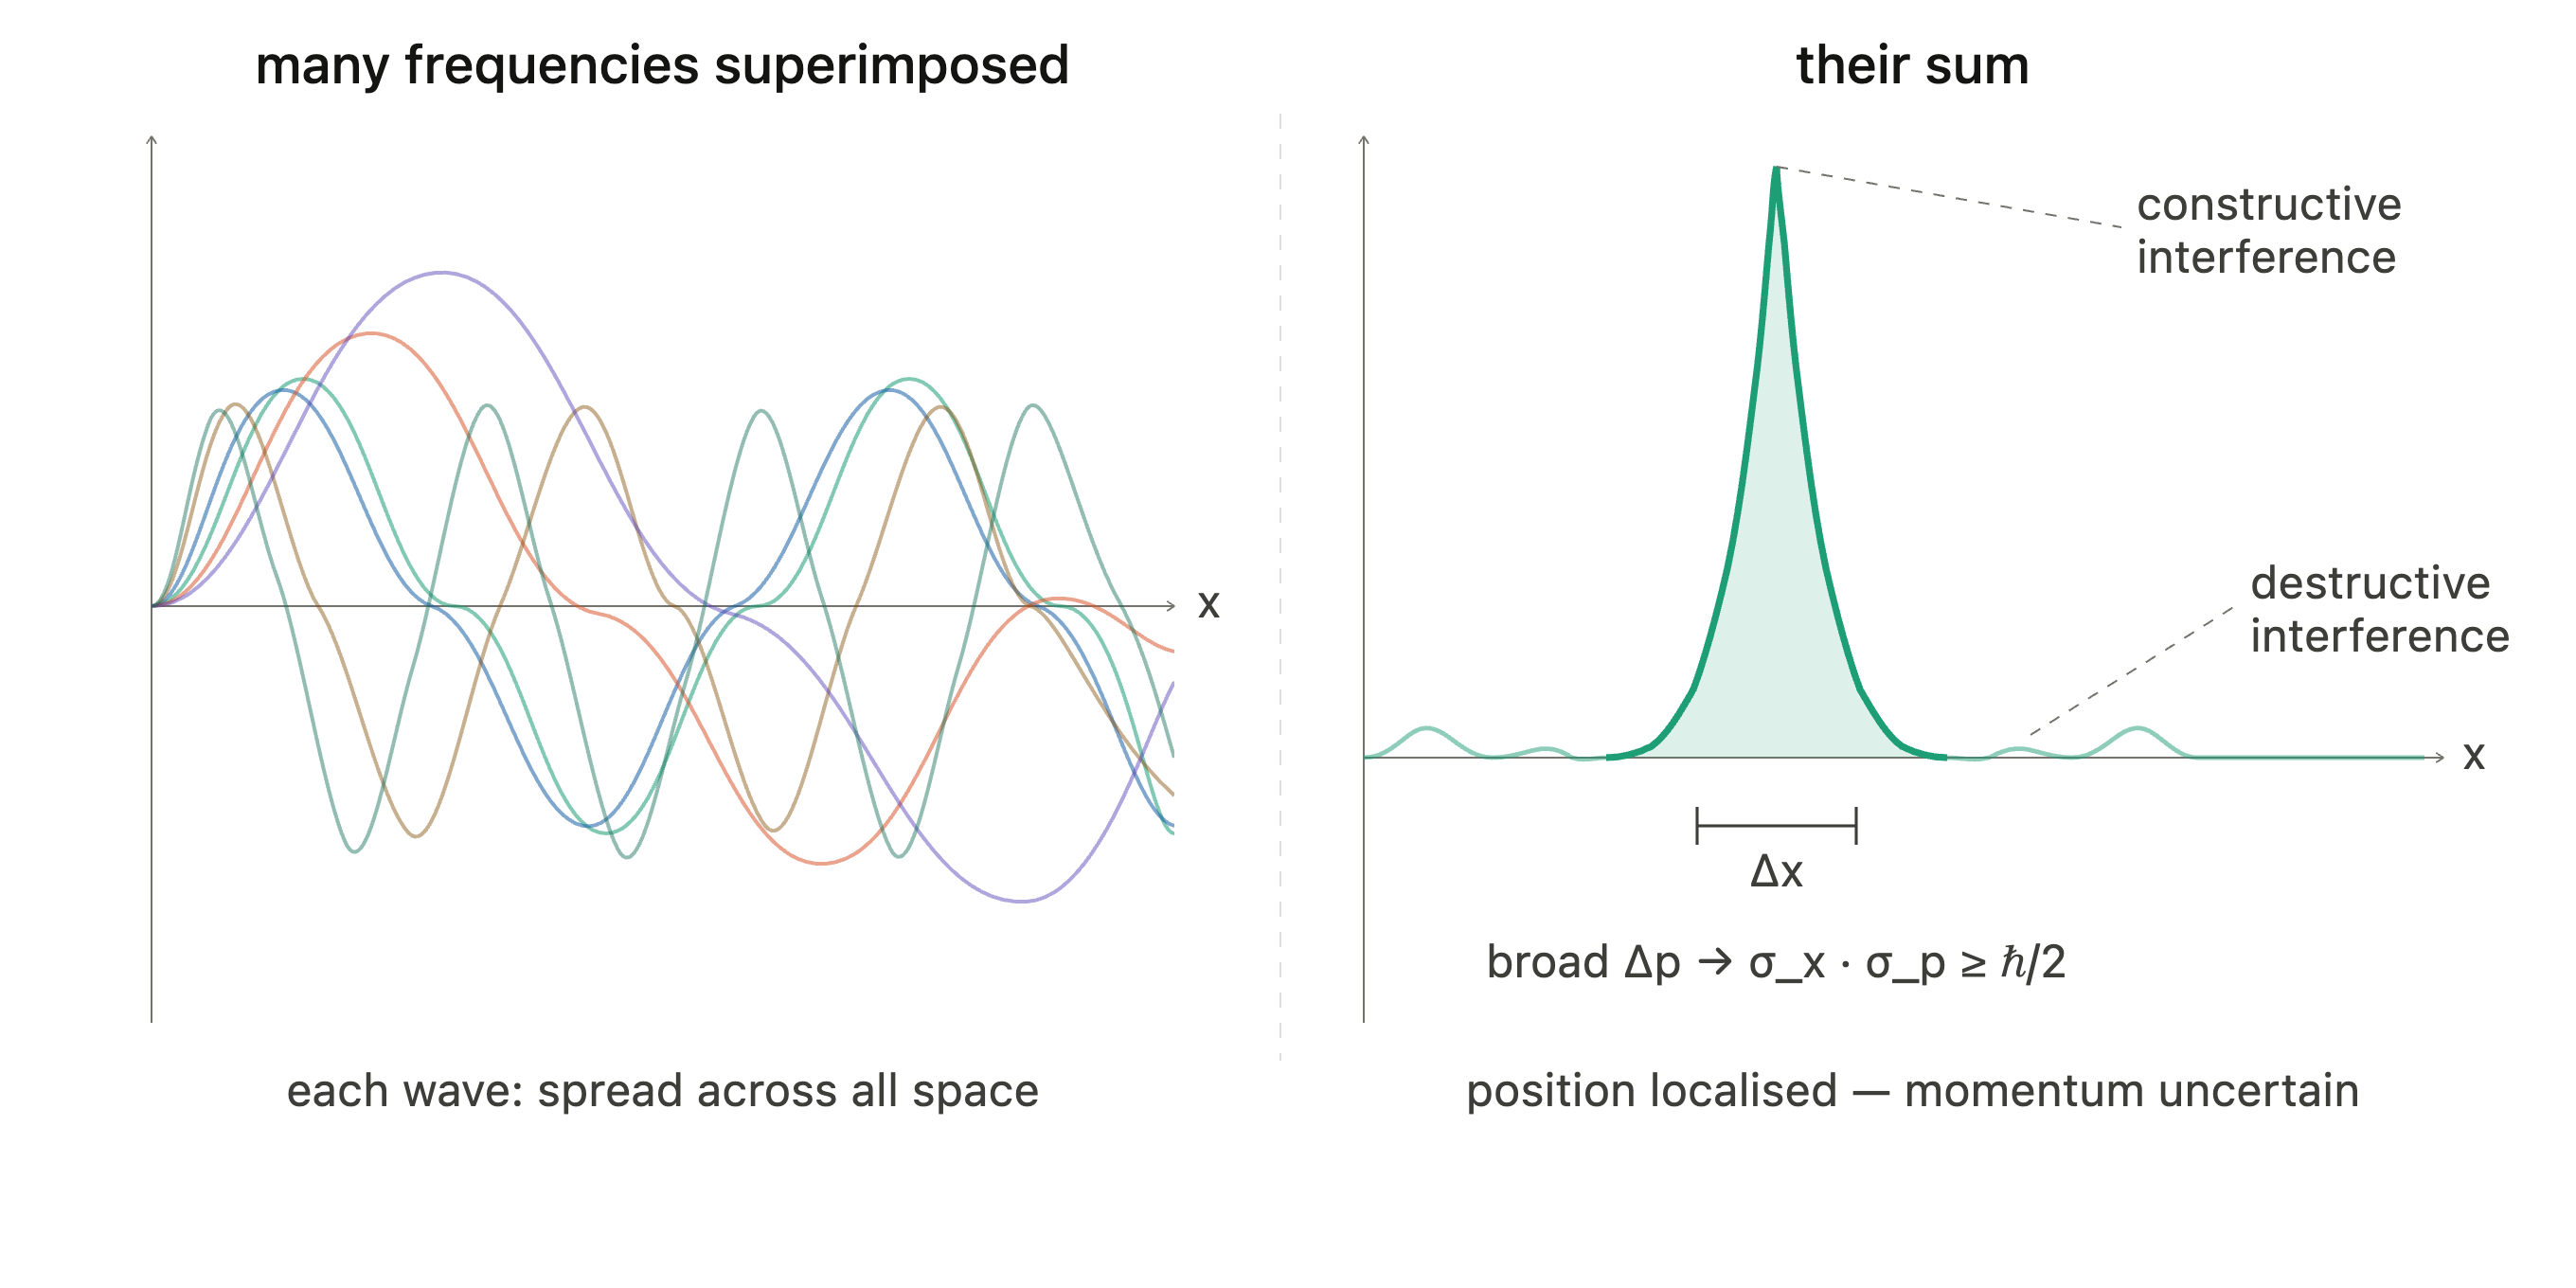
\includegraphics[width=\textwidth]{img/fourier_two_panel.png}
\caption{Left: sine waves of many different frequencies superimposed, each individually delocalised across all space. Right: their sum — constructive interference produces a sharp localised peak while destructive interference suppresses the wave everywhere else. Localising the particle in position space necessarily broadens its distribution in momentum space, so that $\sigma_x \cdot \sigma_p \geq \hbar/2$.}
\label{fig:uncertainty}
\end{figure}

You cannot have both. This is not a limitation of our measuring 
instruments. It is a property of waves.

$$\sigma_x \sigma_p \neq 0$$

The question is: how large must this product be? That is what the 
Kennard inequality tells us.\\

\section*{The Born Ultimatum}

Now it seems we have a full theory of dynamics, except one problem 
remains. If we prepare a particle in a certain position (by, say, 
measuring it), and then measure its momentum, what do we get? 
Certainly not a spectrum of momentum eigenvalues! Answering this 
question, unfortunately, requires speaking to the experimentalists.\\

It turns out that for each measurement, only one eigenvalue is 
recorded, occurring with probability $|\phi(p)|^2$, and similarly 
for position with $|\psi(x)|^2$. A single measurement returns a 
single eigenvalue, chosen at random with probability given by the 
squared amplitude of the corresponding eigenstate:

$$\boxed{P(x) = |\psi(x)|^2 \qquad P(p) = |\phi(p)|^2}$$

This is the Born rule. Everything we have derived so far --- the 
Schr\"{o}dinger equation, the operator formalism, the commutation 
relations --- followed from classical mechanics, Planck's 
quantisation, and the demand for internal consistency. The Born rule 
is different. It cannot be derived. It is the single genuinely 
quantum input, the place where the theory makes contact with 
experiment and refuses to explain itself further.\\

It tells us something profound and uncomfortable: we can only 
interact with part of the quantum world at any one time. The 
wavefunction contains everything there is to know about the system, 
but each measurement extracts only one eigenvalue from it, 
irreversibly and at random. The rest of the information --- the 
full superposition --- is inaccessible.\\

Since the particle must be somewhere, the probabilities must sum 
to one. This fixes the normalisation:

$$\boxed{\int_{-\infty}^{+\infty} \psi^*(x)\psi(x)\,dx = 1}$$

\section*{The Kennard Inequality}

We argued on physical grounds that $\sigma_x\sigma_p \neq 0$. Now 
let us prove the strongest possible version of that statement.\\

Choose coordinates so that the mean position and mean momentum both 
vanish. The variances are then:

$$\sigma_x^2 = \int_{-\infty}^{+\infty} x^2|\psi(x)|^2\,dx 
= \langle\psi|x^2|\psi\rangle$$

$$\sigma_p^2 = \int_{-\infty}^{+\infty} p^2|\phi(p)|^2\,dp 
= \langle\psi|\hat{p}^2|\psi\rangle$$

Define $f(x) = x\psi(x)$ and $g(x) = \hat{p}\psi(x) = 
-i\hbar\frac{d\psi}{dx}$, so that $\sigma_x^2 = \langle f|f\rangle$ 
and $\sigma_p^2 = \langle g|g\rangle$. The Cauchy--Schwarz inequality 
gives:

$$\sigma_x^2\sigma_p^2 = \langle f|f\rangle\langle g|g\rangle 
\geq |\langle f|g\rangle|^2$$

For any complex number $z$:

$$|z|^2 \geq \left(\mathrm{Im}(z)\right)^2 
= \left(\frac{z - z^*}{2i}\right)^2$$

So:

$$|\langle f|g\rangle|^2 \geq 
\left(\frac{\langle f|g\rangle - \langle g|f\rangle}{2i}\right)^2$$

Now we compute $\langle f|g\rangle - \langle g|f\rangle$, which is 
precisely the expectation value of the commutator $[\hat{x}, \hat{p}]$:

$$\langle f|g\rangle - \langle g|f\rangle 
= \langle\psi|[\hat{x},\hat{p}]|\psi\rangle 
= i\hbar\langle\psi|\psi\rangle = i\hbar$$

Substituting everything back:

$$\sigma_x^2\sigma_p^2 \geq 
\left(\frac{i\hbar}{2i}\right)^2 = \frac{\hbar^2}{4}$$

And finally:

$$\boxed{\sigma_x\sigma_p \geq \frac{\hbar}{2}}$$

This is the Heisenberg uncertainty principle, proven rigorously. 
It is not a statement about the clumsiness of measurement. It is 
not an engineering limitation. It is a theorem, following 
inexorably from the single fact that $[\hat{x}, \hat{p}] = i\hbar$ 
--- which itself followed from promoting classical variables to 
operators.\\

The uncertainty is not in our knowledge of the particle. It is 
in the particle itself.\\

\part{Creation and Annihilation}

\section*{Completing the Quantisation}

We have a fully developed theory of quantum dynamics. We have the 
Schr\"{o}dinger equation, the operator formalism, the commutation 
relations, and the Born rule. We know that energy is quantised, 
that position and momentum are irreducibly uncertain, and that the 
classical world emerges from the quantum one in the limit 
$\hbar \to 0$.\\

Naturally, it is only a matter of time before an experimentalist 
screws everything up. In fact, so far we have no description of 
\textbf{spin} --- an intrinsic angular momentum carried by 
particles that has no classical analogue and is not predicted by 
the Schr\"{o}dinger equation. That will require the Dirac equation, 
and we will get there. But as classical physicists we are tired, 
and we have not looked at a mass on a spring in quite some time.\\

So let us return to where we started, and do it properly.\\

\section*{The Classical Oscillator, Revisited}

Before quantising the harmonic oscillator, it is worth pausing to 
look at the classical case from a new angle. Take the Hamiltonian:

$$H = \frac{1}{2\varkappa}q^2 + \frac{1}{2\rho}p^2$$

where $p = \rho\dot{q}$. Hamilton's equations give:

$$\dot{p} = -\frac{q}{\varkappa} \qquad \dot{q} = \frac{p}{\rho}$$

Written as a matrix equation:

$$\frac{d}{dt}\begin{pmatrix}q\\p\end{pmatrix} = 
\begin{pmatrix}0 & 1/\rho \\ -1/\varkappa & 0\end{pmatrix}
\begin{pmatrix}q\\p\end{pmatrix}$$

The matrix on the right is not diagonal, which means $q$ and $p$ 
are coupled --- the evolution of each depends on the other. The 
natural thing to do is find coordinates in which the matrix 
\textit{is} diagonal, so that the equations decouple. We 
rescale to $x = Aq$ and $y = Bp$ with the constraint 
$A/B = \sqrt{\rho/\varkappa}$, which gives:

$$\frac{d}{dt}\begin{pmatrix}x\\y\end{pmatrix} = 
\omega_0\begin{pmatrix}0 & 1 \\ -1 & 0\end{pmatrix}
\begin{pmatrix}x\\y\end{pmatrix}$$

The eigenvectors of this matrix are the combinations that evolve 
independently. They are:

$$\begin{cases}
a = x + iy \quad \text{with eigenvalue } i\omega_0 \\[4pt]
a^* = x - iy \quad \text{with eigenvalue } -i\omega_0
\end{cases}$$

And their time-dependence is beautifully simple:

$$\boxed{\dot{a} = i\omega_0 a \qquad a(t) = a(0)e^{i\omega_0 t}}$$
$$\boxed{\dot{a}^* = -i\omega_0 a^* \qquad a^*(t) = a^*(0)e^{-i\omega_0 t}}$$

Instead of tracking position and momentum separately, we track 
a single complex amplitude $a$ that rotates in the complex plane 
at frequency $\omega_0$. The entire dynamics of the oscillator 
is encoded in this one number.\\

This is the classical version of something we are about to do 
quantum mechanically. The analogy will be exact.\\

\section*{The Quantum Harmonic Oscillator}

The Hamiltonian for the quantum harmonic oscillator is:

$$\hat{H} = \frac{\hat{p}^2}{2m} + \frac{1}{2}m\omega^2\hat{x}^2$$

We want to do the same trick we just did classically --- find 
combinations of $\hat{x}$ and $\hat{p}$ that diagonalise the 
problem. Factor out $\hbar\omega$ and introduce the dimensionless 
operators:

$$\hat{\xi} = \sqrt{\frac{m\omega}{2\hbar}}\,\hat{x} \qquad 
\hat{\eta} = \frac{\hat{p}}{\sqrt{2m\hbar\omega}}$$

so that $\hat{H} = \hbar\omega\left[\hat{\xi}^2 + \hat{\eta}^2\right]$. 
This looks like the sum of two squares, which in ordinary algebra 
we would factor as $(a+ib)(a-ib)$. We try the same here, defining:

$$\begin{cases}
\hat{a} = \hat{\xi} + i\hat{\eta} \\[4pt]
\hat{a}^\dagger = \hat{\xi} - i\hat{\eta}
\end{cases}$$

In terms of the original operators:

$$\boxed{\hat{a} = \sqrt{\frac{m\omega}{2\hbar}}
\left(\hat{x} + \frac{i}{m\omega}\hat{p}\right)}$$

$$\boxed{\hat{a}^\dagger = \sqrt{\frac{m\omega}{2\hbar}}
\left(\hat{x} - \frac{i}{m\omega}\hat{p}\right)}$$

These are the quantum analogues of $a$ and $a^*$ from the 
classical case. But there is a crucial difference: $\hat{x}$ 
and $\hat{p}$ do not commute, so $\hat{a}$ and $\hat{a}^\dagger$ 
are not simply complex conjugates of each other in the classical 
sense. Using $[\hat{\xi}, \hat{\eta}] = \frac{i}{2}$:

$$\begin{cases}
\hat{a}\hat{a}^\dagger = \hat{\xi}^2 + \hat{\eta}^2 
+ i[\hat{\eta},\hat{\xi}] \\[4pt]
\hat{a}^\dagger\hat{a} = \hat{\xi}^2 + \hat{\eta}^2 
- i[\hat{\eta},\hat{\xi}]
\end{cases}$$

Adding and subtracting:

$$\hat{H} = \frac{\hbar\omega}{2}
(\hat{a}\hat{a}^\dagger + \hat{a}^\dagger\hat{a}) 
\qquad [\hat{a},\hat{a}^\dagger] = 1$$

And the Hamiltonian takes its most useful form:

$$\boxed{\hat{H} = \hbar\omega\left(\hat{a}^\dagger\hat{a} 
+ \frac{1}{2}\right)}$$

The operator $\hat{N} = \hat{a}^\dagger\hat{a}$ is called the 
number operator. Its eigenvalues, as we are about to discover, 
count the quanta of energy in the oscillator.\\

\section*{Creation and Annihilation}

Now let us find out what $\hat{a}$ and $\hat{a}^\dagger$ actually 
do to energy eigenstates. Computing their commutators with 
$\hat{H}$:

$$[\hat{H},\hat{a}] = \hbar\omega[\hat{a}^\dagger\hat{a},\hat{a}] 
= \hbar\omega[\hat{a}^\dagger,\hat{a}]\hat{a} = -\hbar\omega\hat{a}$$

$$[\hat{H},\hat{a}^\dagger] = +\hbar\omega\hat{a}^\dagger$$

Suppose $|n\rangle$ is an energy eigenstate with eigenvalue $E_n$. 
Then:

$$\hat{H}(\hat{a}|n\rangle) = \hat{a}\hat{H}|n\rangle 
+ [\hat{H},\hat{a}]|n\rangle 
= (E_n - \hbar\omega)(\hat{a}|n\rangle)$$

$$\boxed{\hat{H}\hat{a}|n\rangle = (E_n - \hbar\omega)\hat{a}|n\rangle 
\qquad \hat{H}\hat{a}^\dagger|n\rangle = 
(E_n + \hbar\omega)\hat{a}^\dagger|n\rangle}$$

$\hat{a}$ takes an energy eigenstate and produces another one 
with energy reduced by exactly $\hbar\omega$. $\hat{a}^\dagger$ 
does the opposite. They destroy and create single quanta of 
energy --- which is why they are called the annihilation and 
creation operators. The energy spectrum is a ladder, with rungs 
spaced exactly $\hbar\omega$ apart:

$$\hat{a}|n\rangle = c_n|n-1\rangle \qquad 
\hat{a}^\dagger|n\rangle = d_n|n+1\rangle$$

\section*{Zero Point Energy}

Repeated application of $\hat{a}$ lowers the energy without 
limit --- unless there is a ground state that it cannot lower 
further. There must be, because $\hat{H}$ has only positive 
eigenvalues. Call this state $|0\rangle$. Applying $\hat{a}$ 
to it must give zero identically, otherwise we could generate 
a state of still lower energy:

$$\hat{a}|0\rangle = 0$$

Applying the Hamiltonian:

$$\hat{H}|0\rangle = \hbar\omega\left(\hat{a}^\dagger\hat{a} 
+ \frac{1}{2}\right)|0\rangle = \frac{1}{2}\hbar\omega|0\rangle$$

The ground state has energy $E_0 = \frac{1}{2}\hbar\omega$, and 
the full spectrum is:

$$\boxed{E_n = \left(n + \frac{1}{2}\right)\hbar\omega \qquad 
n = 0,1,2,\ldots}$$

This is Planck's result, derived from first principles. The 
energy is quantised in units of $\hbar\omega$, exactly as he 
postulated. But there is something Planck did not anticipate: 
the ground state energy is not zero. Even at absolute zero, 
the oscillator retains $\frac{1}{2}\hbar\omega$ of irreducible 
energy. This is the zero-point energy, and it is a direct 
consequence of the uncertainty principle --- a perfectly still 
oscillator would have both definite position and definite 
momentum, which is forbidden.\\

The vacuum is not empty. It fluctuates.\\

\section*{QHO Eigenstates}

We fix the normalisation constants by requiring $|n\rangle$ 
and $|n-1\rangle$ to both be normalised:

$$\langle n|\hat{a}^\dagger\hat{a}|n\rangle = |c_n|^2$$

Since $\hat{a}^\dagger\hat{a} = \hat{N}$ and 
$\hat{N}|n\rangle = n|n\rangle$:

$$|c_n|^2 = n \qquad \Rightarrow \qquad c_n = \sqrt{n}$$

Similarly $d_n = \sqrt{n+1}$, giving:

$$\boxed{\hat{a}|n\rangle = \sqrt{n}\,|n-1\rangle} \qquad 
\boxed{\hat{a}^\dagger|n\rangle = \sqrt{n+1}\,|n+1\rangle}$$

The entire tower of eigenstates is generated by repeated 
application of $\hat{a}^\dagger$ to the ground state. All 
that remains is to find $|0\rangle$ explicitly. In position 
space, $\hat{a}|0\rangle = 0$ becomes a first order 
differential equation:

$$\left(\sqrt{\frac{m\omega}{2\hbar}}\,x 
+ \frac{1}{\sqrt{2m\hbar\omega}}\frac{d}{dx}\right)u_0(x) = 0$$

$$\frac{du_0}{dx} = -\frac{m\omega}{\hbar}\,x\,u_0(x)$$

The solution is a Gaussian:

$$\boxed{u_0(x) = C_0\,\exp\!\left(-\frac{m\omega}{2\hbar}x^2\right)}$$

And the excited states are:

$$\boxed{u_n(x) = \frac{1}{\sqrt{n!}}\,(\hat{a}^\dagger)^n\,u_0(x)}$$

We started with a spring. We ended with a Gaussian ground state 
and a tower of quantised energy levels, each one reachable from 
the last by a single act of creation. The harmonic oscillator 
--- the simplest system in all of physics --- turns out to be 
the skeleton of quantum field theory itself. Every quantum field 
is an infinite collection of these oscillators, one for each 
mode, each with its own ladder of states. The particles we 
observe are the excitations of those ladders.\\

A photon is a quantum of the electromagnetic field. An electron 
is a quantum of the electron field. Creation and annihilation 
are not metaphors.\\

\begin{center}
\textit{It's done.}
\end{center}

\part{Dirac's Coup}

By this point we have built quantum mechanics from the ground up. We
have a wave equation, an operator formalism, a probability
interpretation, and a complete solution to the harmonic oscillator.
The theory is internally consistent, mathematically elegant, and
experimentally confirmed.\\

It is also, as Dirac noticed in 1928, relativistically ugly.\\

\section*{The Problem with Schr\"{o}dinger}

Recall the single particle Schr\"{o}dinger equation:

$$i\hbar\frac{\partial\psi}{\partial t} =
-\frac{\hbar^2}{2m}\nabla^2\psi + V\psi$$

This equation is first order in time but second order in space. From
the perspective of special relativity, this is a problem. Einstein
had shown, following Maxwell's prediction that light travels at $c$
regardless of the observer, that space and time are not separate
things. They are woven together into a single four-dimensional
fabric, and any fundamental equation of physics must treat them on
equal footing.\\

The Schr\"{o}dinger equation does not. It is first order in $t$ and
second order in $\nabla$. It breaks the symmetry that special
relativity demands.\\

The fix seems obvious: find a wave equation that is second order in
both. Klein and Gordon did exactly this, starting from the
relativistic energy-momentum relation:

$$E^2 = p^2c^2 + m^2c^4$$

Substituting the quantum operators $E \to i\hbar\frac{\partial}{\partial t}$
and $\vec{p} \to -i\hbar\nabla$:

$$-\hbar^2\frac{\partial^2\psi}{\partial t^2} =
-\hbar^2c^2\nabla^2\psi + m^2c^4\psi$$

This is the Klein--Gordon equation. It is relativistically covariant
--- space and time appear symmetrically --- and it reduces to the
Schr\"{o}dinger equation in the non-relativistic limit. It seemed
like the answer.\\

But it has a fatal flaw. The probability density derived from the
Klein--Gordon equation is not positive definite. It can go negative.
A negative probability is not a probability at all, and the Born
rule collapses. Klein--Gordon describes something, but not a single
quantum particle.\\

\section*{Dirac's Insight}

Dirac's approach was characteristically audacious. Rather than
accepting the Klein--Gordon equation and trying to fix its
interpretation, he went back to the beginning and asked a sharper
question: is there a wave equation that is first order in both space
and time, and still consistent with the relativistic energy-momentum
relation?\\

The problem is algebraic. We want an operator $\hat{D}$ such that
$\hat{D}^2$ gives back the Klein--Gordon operator. In other words,
we want to take the square root of:

$$\frac{1}{c^2}\frac{\partial^2}{\partial t^2} -
\nabla^2 + \frac{m^2c^2}{\hbar^2}$$

Taking a square root of a differential operator is not something
you can do with ordinary numbers. Dirac realised that if the
coefficients were not numbers but matrices, it might be possible.
He looked for a set of matrices $\gamma^\mu$ satisfying:

$$\gamma^\mu\gamma^\nu + \gamma^\nu\gamma^\mu = 2g^{\mu\nu}$$

where $g^{\mu\nu}$ is the metric of spacetime. This is the Clifford
algebra, and it turns out to have solutions in four dimensions: the
$\gamma$ matrices are $4 \times 4$.\\

The result is the Dirac equation:

$$\boxed{\left(i\gamma^\mu\partial_\mu - \frac{mc}{\hbar}\right)\psi = 0}$$

Or in the equivalent form that makes the Hamiltonian structure
explicit:

$$i\hbar\frac{\partial\psi}{\partial t} =
\left(-i\hbar c\,\vec{\alpha}\cdot\nabla + \beta mc^2\right)\psi$$

where $\vec{\alpha}$ and $\beta$ are $4 \times 4$ matrices built
from the $\gamma^\mu$. This equation is first order in both space
and time, relativistically covariant, and has a positive definite
probability density.\\

It is the most beautiful equation in physics.\\

\section*{The Gift Nobody Asked For}

Now for the miracle. The wavefunction $\psi$ that solves the Dirac
equation is not a scalar, and not a three-component vector. It is a
four-component object called a spinor, because the $4 \times 4$
matrix structure of the equation forces it to have four independent
components.\\

Two of these components correspond to the particle --- the electron,
say --- with two possible internal states. Dirac did not put these
states in by hand. He did not postulate them. They simply fell out
of the algebra, as an inevitable consequence of demanding that
quantum mechanics be consistent with special relativity.\\

Those two internal states are the spin-up and spin-down states of
the electron. Spin --- the intrinsic angular momentum that has no
classical analogue, that cannot be explained by any picture of a
spinning ball, that had been observed experimentally for years
without theoretical justification --- is not an additional
assumption of quantum mechanics. It is a prediction of it.\\

You get it for free, the moment you insist that your wave equation
treat space and time equally.\\

\section*{The Other Two Components}

The remaining two components of the spinor are stranger still.
Dirac initially tried to interpret them away, but the mathematics
refused. They correspond to solutions with negative energy ---
states that seemed to have no physical meaning.\\

Rather than discard them, Dirac proposed something extraordinary.
He imagined that all negative energy states were already filled,
forming an invisible sea of electrons. A hole in this sea --- a
missing negative-energy electron --- would behave like a positive
energy particle with positive charge. He predicted the existence
of the antielectron.\\

In 1932, Carl Anderson found it in a cloud chamber. He called it
the positron.\\

Dirac had set out to fix an aesthetic problem with the
Schr\"{o}dinger equation. He ended up predicting antimatter.\\

\section*{Where We Stand}

We started with a spring. We found that its equation of motion has
wave-like solutions. We found that an infinite chain of springs
becomes a field, and that fields are the natural language of
electromagnetism. We found that particles, taken seriously as
waves, obey the Schr\"{o}dinger equation --- which contains
Hamilton--Jacobi in the classical limit, and reduces to Newton
in the limit $\hbar \to 0$. We quantised the oscillator and
recovered Planck's spectrum. And now we have demanded that all
of this be consistent with special relativity, and the universe
has handed us spin, antimatter, and the most beautiful equation
in physics.\\

Two experimental inputs. A spring. And just following the logic
wherever it goes.\\

\section*{A Note on Beauty}

What we have built in this book is a particular moment in the
history of physics. It spans roughly 1680 to 1930 --- from Newton's
apple to Dirac's spinor --- and it has a quality that is difficult
to name but impossible to miss. It feels finished. The pieces fit
together with an almost unreasonable elegance: a spring becomes a
field, a field becomes a wave, a wave becomes a particle, a particle
becomes a spinor. Each step follows from the last with something
approaching inevitability.\\

This feeling is not an illusion, but it does turn out to be a luxury.\\

After 1930, physics gets harder and considerably messier. Quantum
field theory --- the full machinery of creation and annihilation
operators applied to relativistic fields --- works extraordinarily
well, but it works by a process that Dirac himself found
philosophically repugnant: renormalisation, the systematic
discarding of infinities that appear in the calculations. The
answers are right. The justification is uncomfortable.\\

The Standard Model of particle physics, which describes all known
fundamental particles and three of the four fundamental forces, is
the most precisely tested theory in the history of science. It is
also, by any aesthetic standard, a mess. It has nineteen free
parameters that must be measured rather than derived. It does not
include gravity. It offers no explanation for dark matter, dark
energy, or the asymmetry between matter and antimatter that allowed
the universe to exist at all.\\

General relativity --- Einstein's theory of gravitation, which we
have not touched --- is arguably as beautiful as anything in this
book. But nobody knows how to make it compatible with quantum
mechanics. The two theories, each internally consistent and
experimentally confirmed to extraordinary precision, simply refuse
to speak the same language. Somewhere at the Planck scale, where
quantum effects and gravitational effects become simultaneously
important, our understanding breaks down completely.\\

String theory, loop quantum gravity, and a dozen other frameworks
have been proposed to bridge the gap. None has produced a
testable prediction that distinguishes it from its rivals. The
question of what happens at the bottom of things remains, for now,
genuinely open.\\

So the snapshot this book has taken --- from the harmonic oscillator
to the Dirac equation --- may be as beautiful as physics ever gets.
The problems that remain are harder, the mathematics is less forgiving, and the constructs we use are further from human intuition than
even anything we have encountered here.\\

What we have shown is that the universe, at least in this corner
of its history, was willing to be understood.\\

Whether that continues to be true, at deeper scales and higher
energies, is the question that will occupy physicists for the rest
of this century. The answer, whatever it turns out to be, will
almost certainly be stranger than anything in this book.\\

That, at least, is something to look forward to.\\


%\bibliographystyle{plain}
%\bibliography{bibtex_example}

\printindex

\end{document}
